\documentclass[a4paper]{article}

\usepackage{polski}
\usepackage[utf8]{inputenc}
\usepackage[pdftex]{graphicx}
\usepackage{fancyhdr}
\usepackage{float}

\newcommand{\prog}{\texttt}

\linespread{1.15}
\pagestyle{fancy}
\fancyhf{}
\chead{Specyfikacja funkcjonalna}
\cfoot{Strona \thepage \ z \pageref{end}}

\title{Specyfikacja funkcjonalna\\Projekt \textit{Aplikacja OnePass} w języku Python}
\author{Jakub Czajka (299239)\\}

\begin{document}

\maketitle
\tableofcontents
\thispagestyle{empty}

\section{Opis ogólny}

\subsection{Nazwa programu}
Jako nazwę programu przyjąłem wyrażenie \prog{OnePass}, które można przetłumaczyć jako \textit{One Password}, co z języka angielskiego oznacza \textit{Jedno hasło}. Jest to ścisłe nawiązanie do funkcjonalności programu, który wymaga od nas pamiętania wyłącznie jednego hasła.

\subsection{Poruszany problem}
\textit{OnePass} jest okienkową aplikacją przeznaczoną na komputery stacjonarne. Aplikacja realizuję usługę menadżera haseł. Aplikacja inspirowana jest aplikacjami typu \textit{KeePass}, \textit{1Password} lub \textit{LastPass}.\\ \\
Użytkowanie rozpoczyna się od utworzenia konta przez podanie danych osobowych, danych kontaktowych oraz hasła, które musi spełniać najnowsze standardy bezpieczeństwa. Następnie przenoszeni jesteśmy do głównego okna aplikacji. Tam możemy rozpocząć dodawanie haseł oraz możemy skorzystać z innych usług dostarczanych przez aplikację. Wszystkie hasła składowane w aplikacji zostają szyfrowane przez co dostęp do nich z poza aplikacji jest niemożliwy. \\ \\
Aplikacja dostarcza usługę generowania haseł, które następnie można skopiować i wykorzystać. W celu wygenerowania haseł użytkownik znajdujący się na ekranie głównym kilka w odpowiednią ikonę na pasku. Po kliknięciu otwierane jest okno pozwalające utworzyć hasło z podanych kryteriów. \\ \\
Oprócz tego aplikacja umożliwia szyfrowanie plików tekstowych podanych przez użytkownika oraz tworzenie szyfrowanych notatek w samej aplikacji. \textit{OnePass} umożliwia również korzystanie z niego wielu użytkownikom. 

\subsection{Użytkownik docelowy}
Program dedykowany jest użytkownikom w dowolnym wieku pragnącym poprawić swoje bezpieczeństwo w sieci przez zmianę haseł na odpowiednio trudne do~złamania lub pragnących pamiętać wyłącznie jedno hasło.

\section{Opis funkcjonalności}
\subsection{Jak korzystać z programu?}
Program należy uruchomić za pomocą kliknięcia na odpowiednią ikonę pliku w~formacie EXE.

\subsection{Uruchomienie programu}
Program posiada graficzny interfejs użytkownika. Po uruchomieniu należy zalogować się lub utworzyć nowe konto.

\subsection{Możliwości programu}
\begin{enumerate}
    \item Utworzenie nowego użytkownika.
    \item Haszowanie hasła.
    \item Wczytanie zapisanego pliku z danymi użytkownika.
    \item Sprawdzenie poprawności danych logowania.
    \item Blokowanie konta w przypadku zbyt dużej liczby prób logowania.
    \item Dodanie nowego pola z hasłami.
    \item Zaszyfrowanie plików algorytmem symetrycznym.
    \item Odszyfrowanie pliku zaszyfrowanego algorytmem symetrycznym.
    \item Wczytanie pliku tekstowego.
    \item Obsługiwanie błędów powstałych przy wczytywaniu plików.
    \item Generacja haseł przy podanych kryteriach.
    \item Tworzenie notatek w aplikacji.
    \item Analizowanie trudności haseł.
\end{enumerate}

\section{Format danych i struktura plików}

\subsection{Pojęcia}
\begin{description}
    \item[Użytkownik]-- osoba używająca program.
    \item[Konto]-- zpersonalizowany profil użytkownika.
    \item[Standardy bezpieczeńswa]-- standardy mówiącę, że hasło ma być długie i skoplikowane.
    \item[Hasło skomplikowane]-- hasło nie zawierające słów możliwych do znalezienia w słowniku. Składa się z małych i dużych liter oraz ze znaków specjalnych.
\end{description}

\subsection{Struktura katalogów}
Drzewo katalogów i plików prezentuje się w następujący sposób:
\begin{itemize}
    \item docs \textit{(miejsce przechowywania dokumentacji programu)}
    \begin{itemize}
        \item[•] img \textit{(miejsce przechowywanie grafiki do dokumentacji)}
    \end{itemize}
    \item sample \textit{(miejsce przechowywania pakietów}
    \begin{itemize}
        \item[•] view \textit{(miejsce przechowywania modułów GUI)}
        \item[•] presenter \textit{(miejsce przechowywania modułów kontrolerów)}
        \item[•] model \textit{(miejsce przechowywania modułów obliczeń)}
    \end{itemize}
    \item tests \textit{(miejsce przechowywania modułów testów jednostkowych)}
    \item data \textit{(miejsce przechowywania danych)}
    \item[--] requirements.txt \textit{(plik przechowujący zależności potrzebne do projektu)}
    \item[--] setup.py
    \item[--] README.md
\end{itemize}

\subsection{Przechowywanie danych w programie}
Pliki będę przechowywał w projektowym repozytorium kontroli wersji Git na platformie GitHub.\\ \\
Dane w programie znajdują się w zmiennych o różnych modyfikatorach dostępu.

\subsection{Dane wejściowe}
Program uwzględnia wczytywanie trzech plików tekstowych. Pliku konfiguracyjnego podczas uruchomienia programu, co odbywa się niejawnie, pliku z danymi konta po zalogowaniu się użytkownika, co również odbywa się niejawnie oraz pliku tekstowego podanego przez użytkownika do zaszyfrowania.

\subsubsection{Plik konfiguracyjny}\label{pKonf}
Plik tekstowy przechowujący konfigurację programu jest plikiem zaszyfrowanym. Po odszyfrowaniu dane znajdują się w następującej postaci:\\ \\
\prog{LoginUżytkownika1;ZahaszowaneHasłoUżytkownika1\\LoginUżytkownika2;ZahaszowaneHasłoUżytkownika2\\...\\LoginUżytkownikaN;ZahaszowaneHasłoUżytkownikaN}

\subsubsection{Plik użytkownika}\label{pUzy}
Plik tekstowy przechowujący dane użytkownika w formie zaszyfrowanej. Po odszyfrowaniu dane znajdują się w następującej postaci:\\ \\
\prog{Imię;Nazwisko;Email;Login;ZahaszowaneHasło\\NazwaObiektu1;LoginDoObiektu1;HasłoDoObiektu1;TypObiektu1;FlagaCzyObiektUlubiony1\\NazwaObiektu2;LoginDoObiektu2;HasłoDoObiektu2;TypObiektu2;FlagaCzyObiektUlubiony2\\...\\NazwaObiektuN;LoginDoObiektN;HasłoDoObiektuN;TypObiektuN;FlagaCzyObiektUlubionyN}

\subsection{Dane wyjściowe}
Program zapisuje pliki wymienione w punktach \ref{pKonf} i \ref{pUzy} wcześniej je szyfrując. Program umożliwia również zaszyfrowanie pliku podanego przez użytkownika. W takim przypadku w pliku znajduje się zaszyfrowana zawartość wpisywana ciągiem.

\section{Scenariusz działania programu}

\subsection{Scenariusz ogólny}
\begin{enumerate}
    \item Uruchomienie programu.
    \item Wybranie opcji:\label{eGłówny}
    \begin{enumerate}
        \item Zaloguj się-- wyświetlone zostaje okno z możliwością wpisania danych do logowania.
        \begin{enumerate}
            \item Uzupełnienie danych.
            \item Zalogowanie na profil.
            \item Wyświetlenie ekranu \textit{Home}
        \end{enumerate}
        \item Zarejestruj się -- wyświetlone zostaje okno z możliwością uzupełnienia formularza do rejestracji.
        \begin{enumerate}
            \item Uzupełnienie danych.
            \item Zarejestrowanie się
            \item Wyświetlenie ekranu \textit{Home}
        \end{enumerate}
        \item Generuj -- wyświetlone zostaje okno z możliwością wygenerowania hasła.\label{gen}
        \begin{enumerate}
            \item Ustawienie kryteriów.
            \item Wygenerowanie hasła
        \end{enumerate}
        \item O aplikacji - wyświetlone zostaje okno z informacjami na temat aplikacji.
    \end{enumerate}
    \item Wybranie opcji:
    \begin{enumerate}
        \item Hasła -- wyświetlone zostaje na ekranie głównym lista  obiektów dodanych do aplikacji
        \begin{enumerate}
            \item Wybranie opcji:
            \begin{enumerate}
                \item Dodaj -- wyświetlone zostaje okno z możliwością dodania nowego obiektu.
                \item Wybierz -- wyświetlone zostaje okno z danymi obiektu.
            \end{enumerate}
        \end{enumerate}
        \item Notatki -- wyświetlona zostaje na ekranie głównym lista notatek znajdujących się w folderu z notatkami aplikacji.
        \begin{enumerate}
            \item Wybranie opcji:
            \begin{enumerate}
                \item Dodaj -- wyświetlone zostaje na ekranie głównym okno z możliwością utworzenia nowej notatki.
                \item Edytuj -- wyświetlone zostaje na ekranie głównym okno z możliwością edytowania notatki.
                \item Po wybraniu którejś z opcji wyświetlone zostaje okno z możliwością edycji notatki oraz możliwością usunięcia notatki
            \end{enumerate}
        \end{enumerate}
        \item Generuj -- otworzone zostaje okno z punktu \ref{gen}
        \item Szyfruj -- wyświetlone zostaje na ekranie głównym okno z możliwością wyboru pliku do zaszyfrowania/odszyfrowania.
        \begin{enumerate}
            \item Wybranie opcji:
            \begin{enumerate}
                \item Zaszyfruj -- plik podany zostaje zaszyfrowany.
                \item Deszyfruj -- plik podany zostaje rozszyfrowany.
            \end{enumerate}
        \end{enumerate}
    \end{enumerate}
    \item Wybranie opcji \textit{Zaszyfruj}.
    \item Aplikacja szyfruje, a następnie nadpisuje wszystkie dane z aplikacji.
    \item Wybranie opcji \textit{Wyloguj}.
    \item Wyświetlenie ekranu omawianego w punkcie \ref{eGłówny}
    \item Zakończenie działania programu.
\end{enumerate}

\newpage

\subsection{Scenariusz szczegółowy}

\subsubsection{Scenariusz wyświetlenia menu} \label{wMenu}
\begin{enumerate}
    \item Użytkownik uruchamia programu.
    \item System rozszyfrowuję plik konfiguracyjny.
    \item System analizuje plik konfiguracyjny
    \item System wyświetla ekran główny przed zalogowaniem.
\end{enumerate}

\subsubsection{Scenariusz zalogowania się}
\begin{enumerate}
    \item Po wykonaniu poleceń z punktu \ref{wMenu}, użytkownik klika przycisk \textit{Zaloguj się}.
    \item System wyświetla ekranu logowania. \label{ekranLog}
    \item Użytkownik uzupełnia dane.
    \begin{itemize}
        \item Użytkowanik klika przycisk \textit{Zaloguj}.
            \begin{enumerate}
                \item System sprawdza dane:
                \begin{itemize}
                    \item[•] Dane poprawne:
                    \begin{enumerate}
                        \item System wyświetla  komunikatu o poprawnym zalogowaniu.
                        \item System rozszyfrowuje plik użytkownika.
                        \item System załadowuje plik użytkownika do programu.
                        \item System wyświetla ekran główny po zalogowaniu się.
                    \end{enumerate}
                    \item[•] Dane niepoprawne:
                    \begin{enumerate}
                        \item System wświetla komunikatu o niepoprawnych danych logowania.
                        \item Powrót do punktu \ref{ekranLog}. wykonywany maksymalnie trzy razy. Przy trzecim razie następuje blokada konta.
                    \end{enumerate}
                \end{itemize}
            \end{enumerate}
        \item Użytkowanik klika przycisk \textit{Nie pamiętasz hasła?}.
        \begin{enumerate}
            \item System zczytuje login.
            \item System rozszyfrowuje plik użytkownika.
            \item System załadowuje zawartość pliku użytkownika.
            \item System wysyła maila z instrukcjami do zresetowania hasła.
        \end{enumerate}
        \item Użytkowanik klika przycisk \textit{Załóż konto}.
        \begin{enumerate}
            \item System wyświetla ekran rejestracji.
        \end{enumerate}
    \end{itemize}
\end{enumerate}

\subsubsection{Scenariusz rejestracji}
\begin{enumerate}
    \item Po wykonaniu poleceń z punktu \ref{wMenu}, użytkownik klika przycisk \textit{Zarejestruj się}.
    \item System wyświetla ekranu rejestracji. \label{ekranRej}
    \item Użytkownik uzupełnia dane.
    \item Użytkowanik klika przycisk \textit{Zarejestruj}.
    \item System sprawdza dane:
    \begin{itemize}
        \item Dane poprawne:
        \begin{enumerate}
            \item System wyświetla  komunikatu o poprawnym zarejestrowaniu.
            \item System tworzy plik użytkownika.
            \item System wyświetla ekran główny po zalogowaniu się.
        \end{enumerate}
        \item Dane niepoprawne:
        \begin{enumerate}
            \item System wświetla komunikatu o niepoprawnych danych.
            \item Powrót do punktu \ref{ekranRej}.
        \end{enumerate}
    \end{itemize}
\end{enumerate}

\subsubsection{Scenariusz dodawania haseł}
\begin{enumerate}
    \item Użytkownik klika przycisk odpowiadający za dodanie nowego obiektu do listy haseł.
    \item System wyświetla okno dodania nowego obiektu haseł.\label{noweH}
    \item Użytkownik uzupełnia dane obiektu.
    \item System sprawdza dane:
    \begin{itemize}
        \item Dane poprawne:
        \begin{enumerate}
            \item System wyświetla  komunikatu o poprawnym utworzeniu obiektu.
            \item System aktualizuję listę haseł.
            \item System wyświetla ekran haseł.
        \end{enumerate}
        \item Dane niepoprawne:
        \begin{enumerate}
            \item System wświetla komunikatu o niepoprawnych danych.
            \item Powrót do punktu \ref{noweH}.
        \end{enumerate}
    \end{itemize}
\end{enumerate}


\newpage

\subsection{Ekrany działania programu}
\paragraph{}Rysunek \ref{fig:startPrzed}. prezentuje ekran startowy programu przed zalogowaniem się użytkownika. Widoczne są na nim 4 ikony pozwalające rozpocząć działanie programu.
\begin{figure}[H]
    \centering
    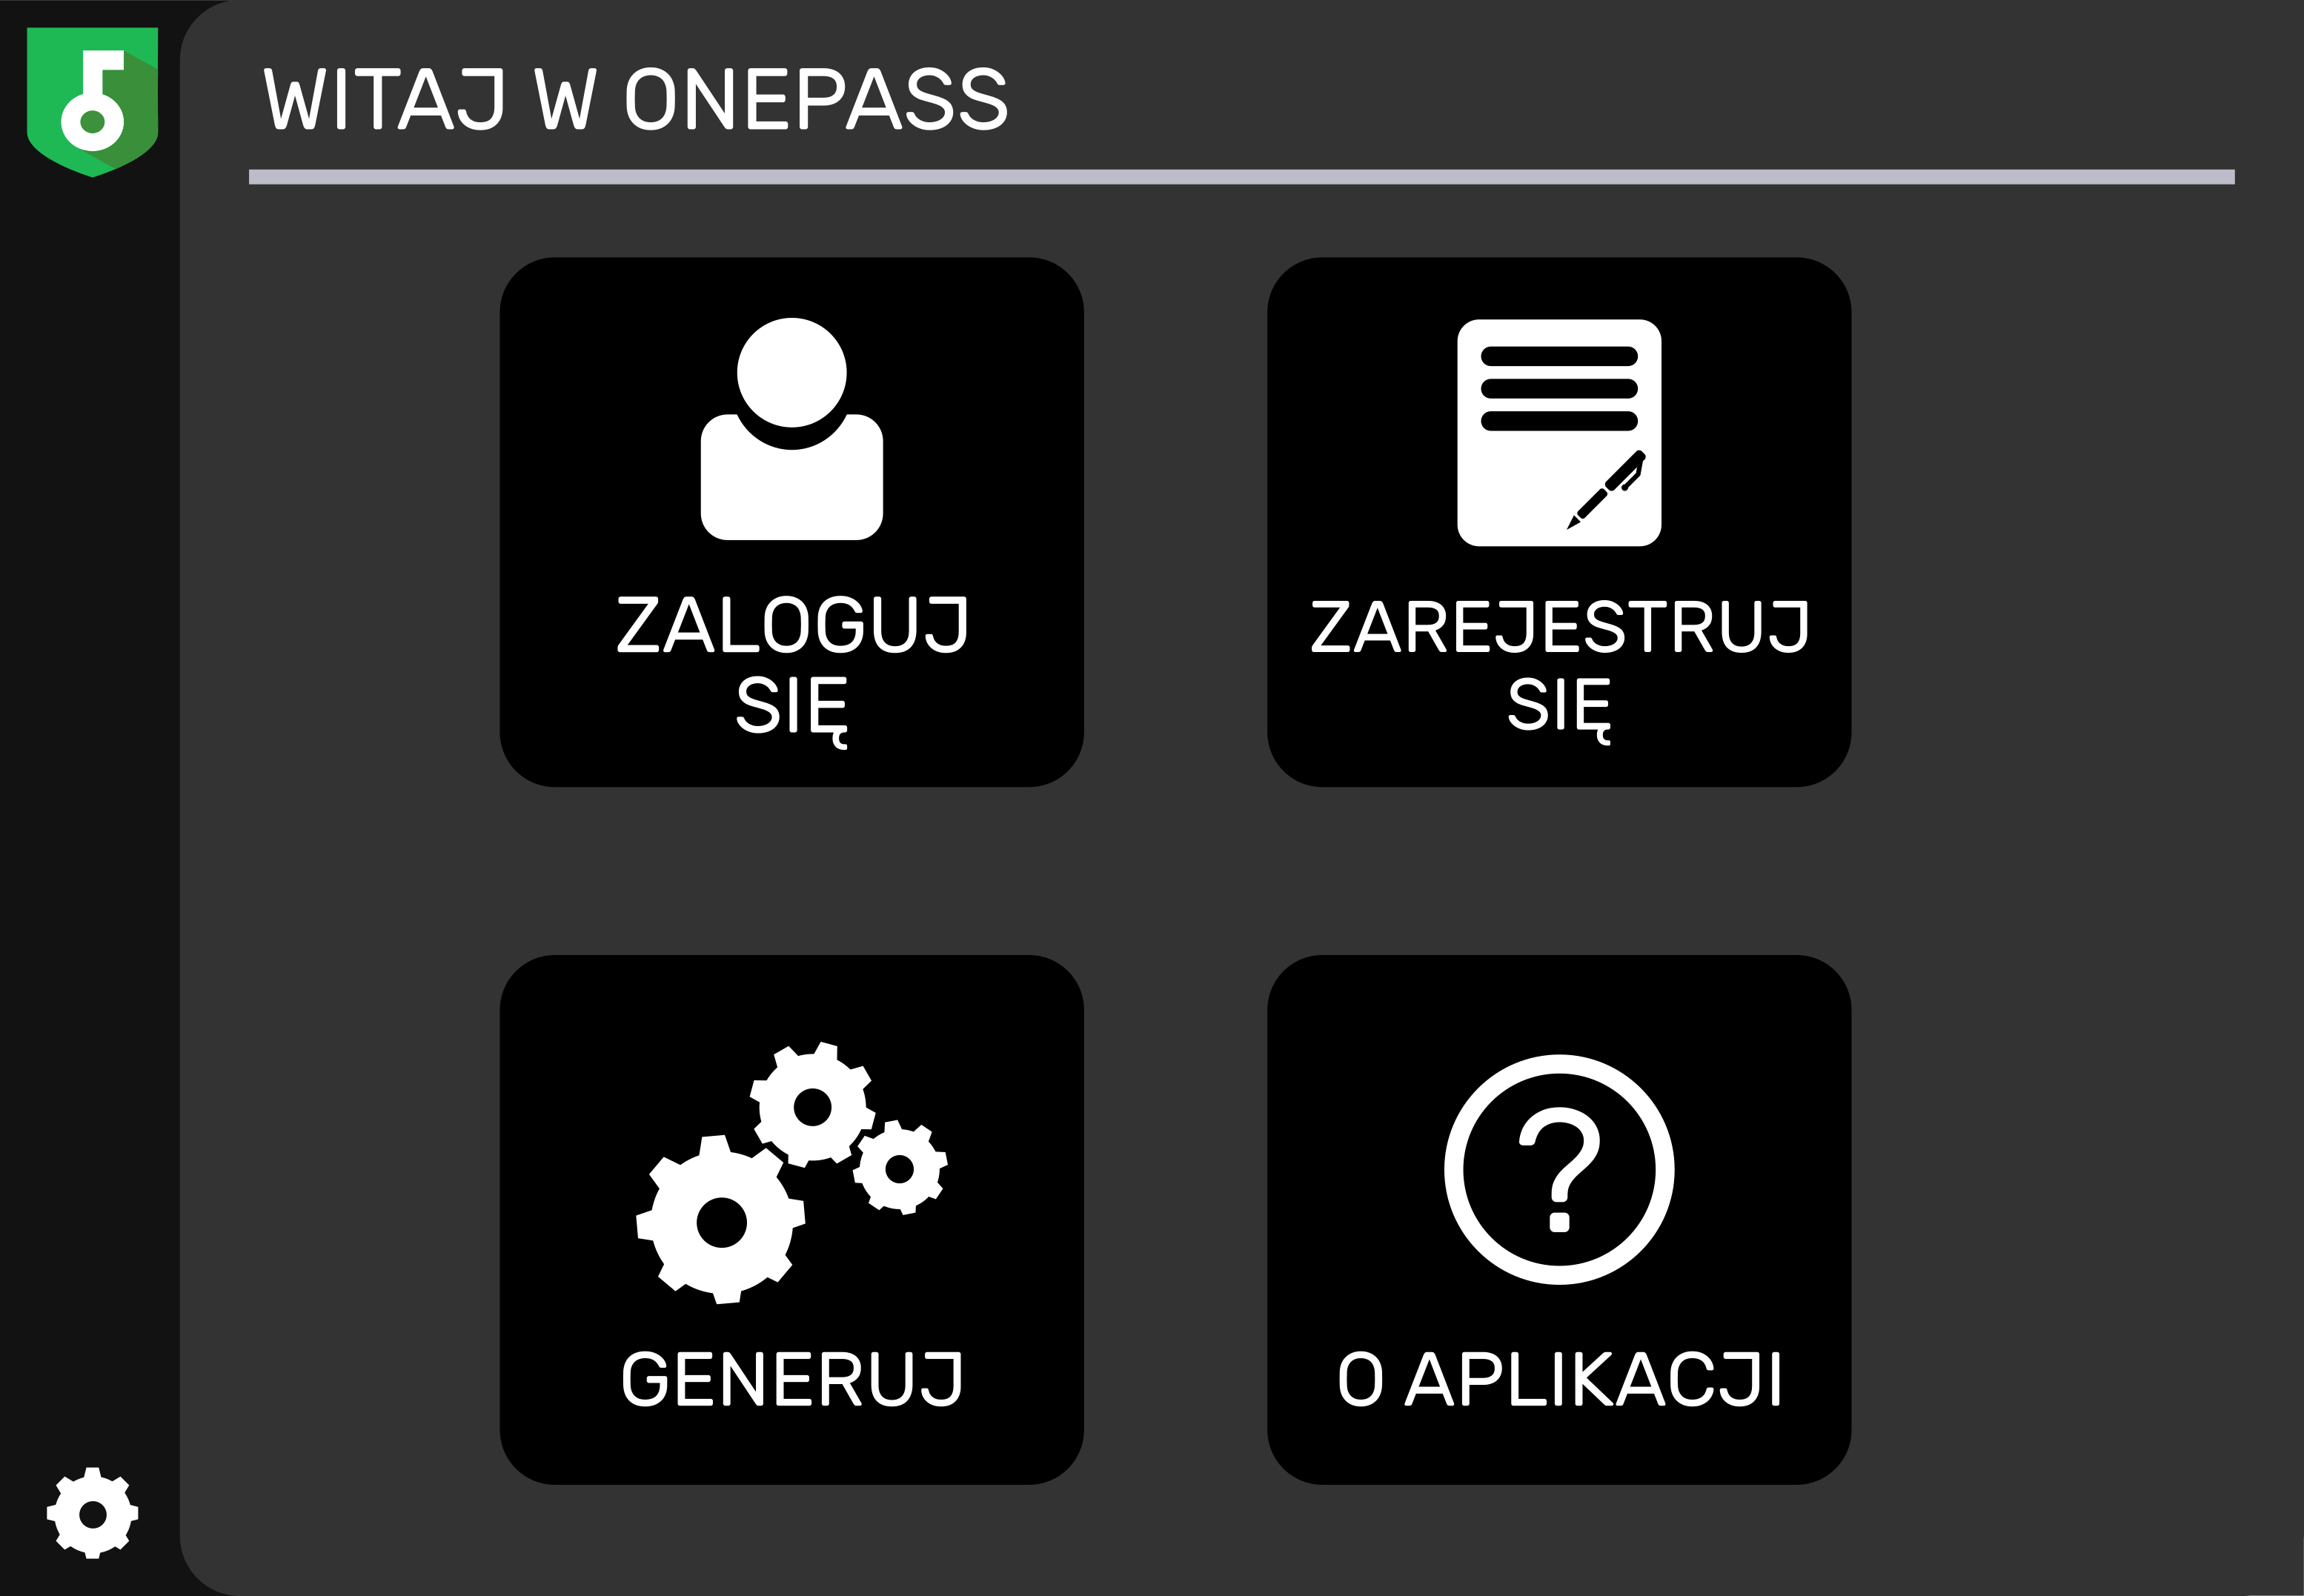
\includegraphics[width=1\textwidth]{img/ekran_przed_zalogowaniem.png}
    \caption{Ekran startowy -- przed zalogowaniem}
    \label{fig:startPrzed}
\end{figure}

\newpage

\paragraph{}Ekran na rysunku \ref{fig:logowanie}. przedstawia wygląd ekranu logowania się użytkownika. Z tego ekranu można przejść do okna rejestracji i można uruchomić mechanizm przypominania hasła. Po kliknięciu przyciku \textit{Zaloguj} zostaniemy przeniesieni do ekranu z rysunku \ref{fig:startPo}.
\begin{figure}[H]
    \centering
    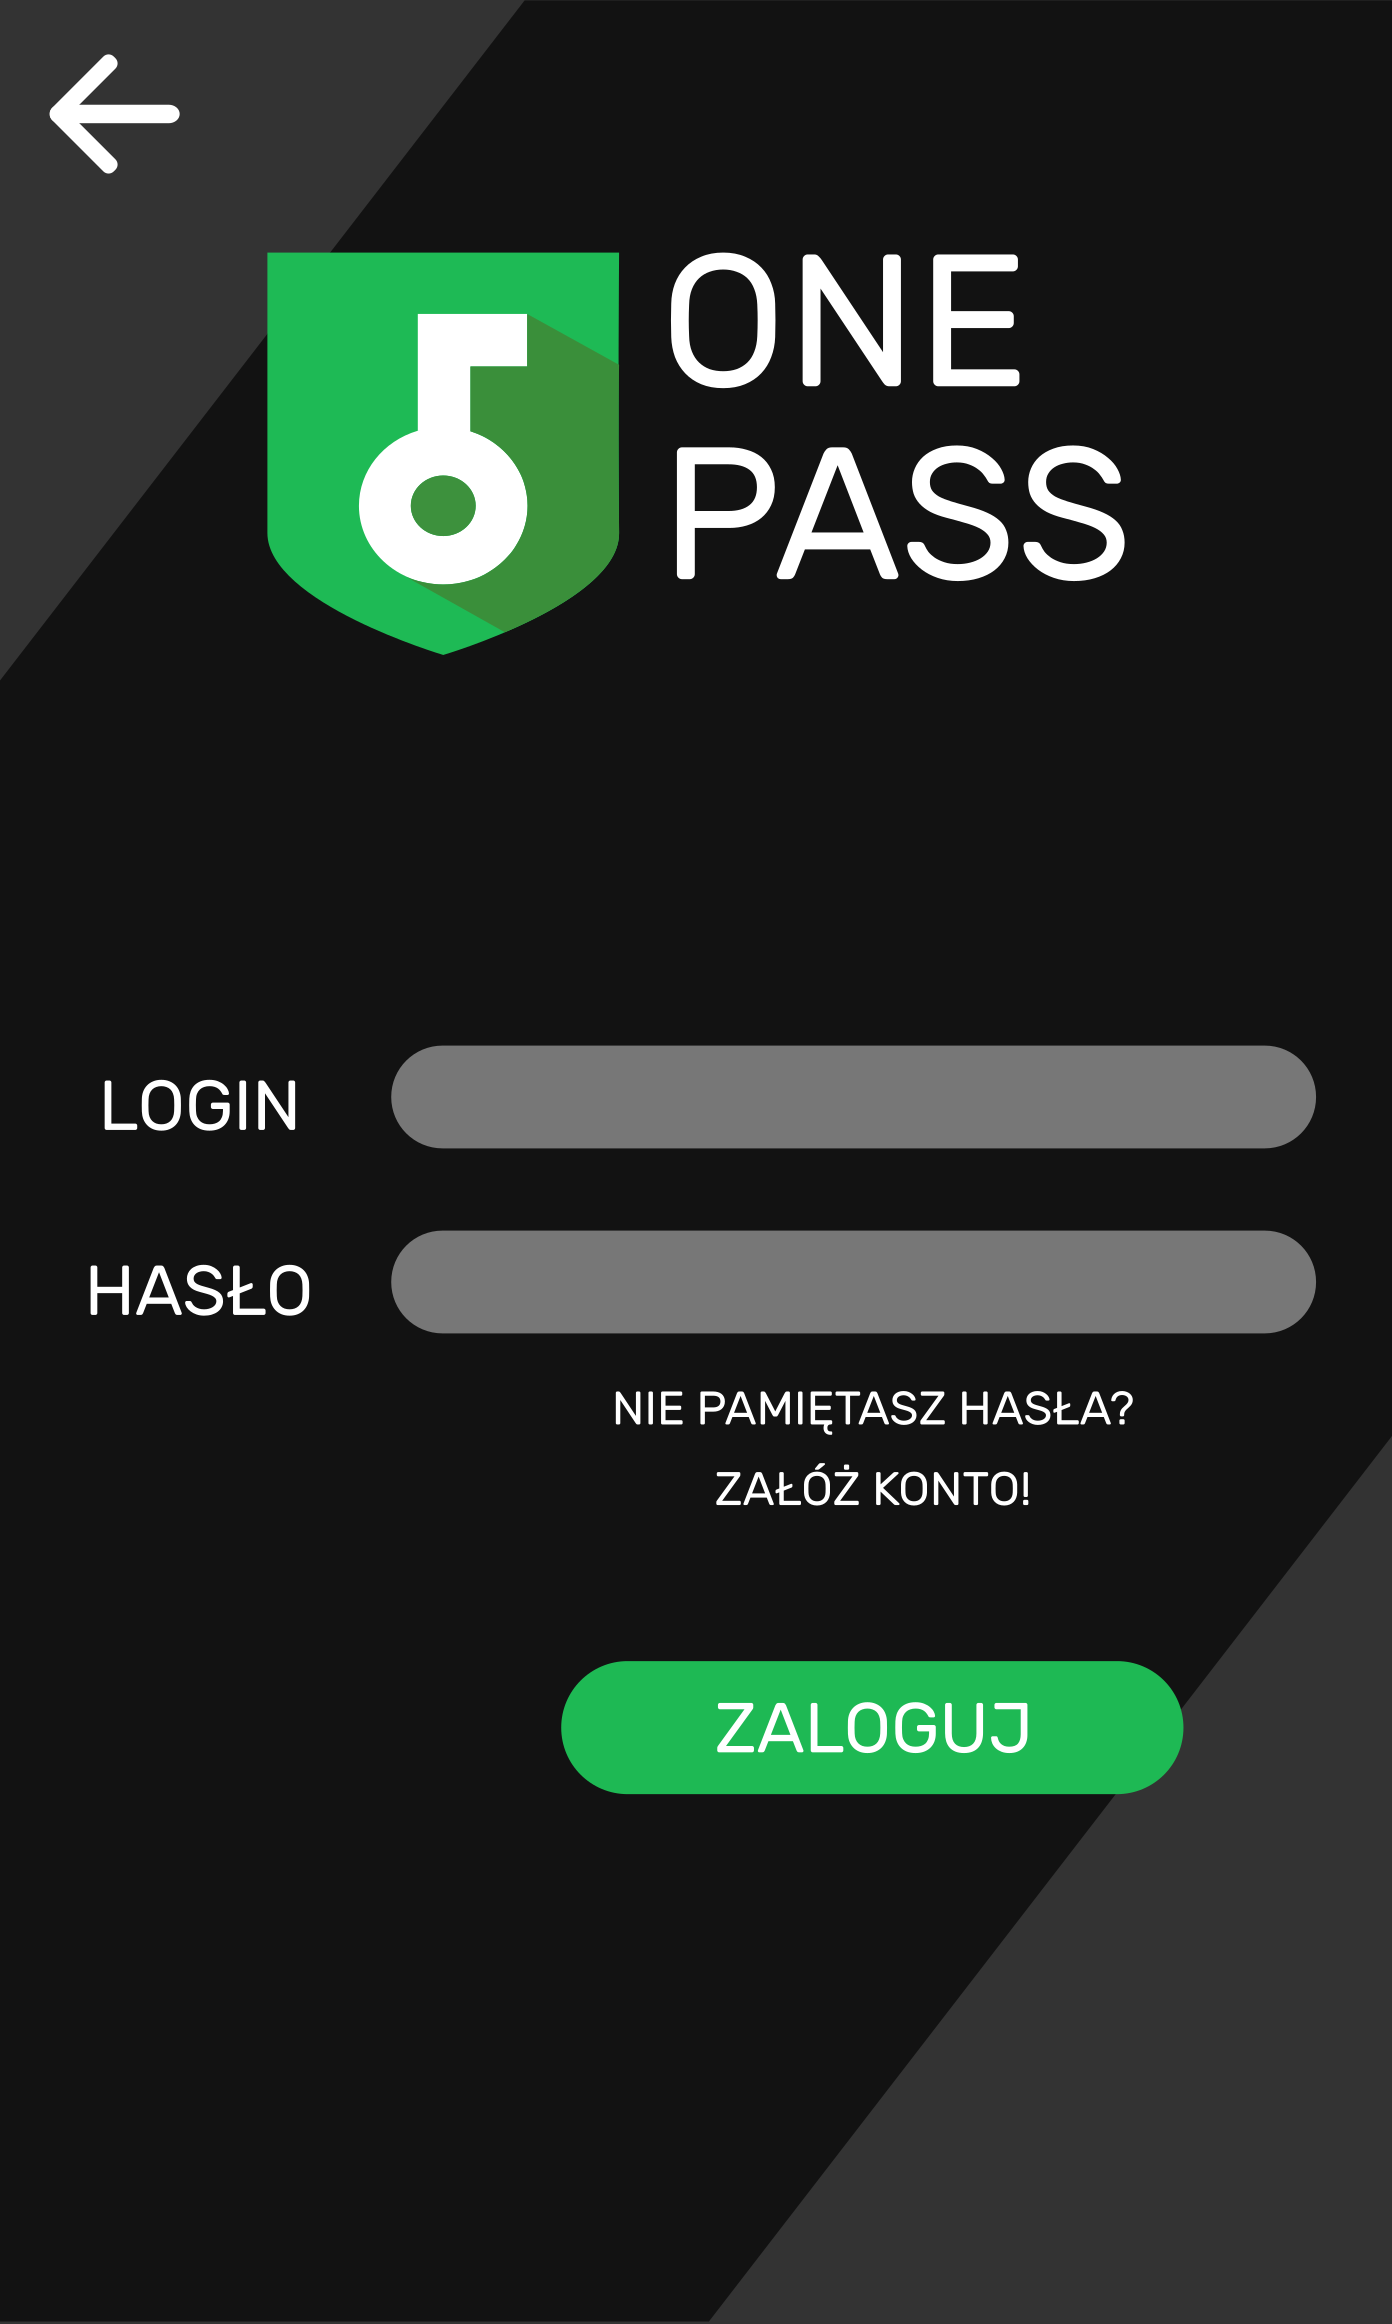
\includegraphics[height = 1\textwidth]{img/ekran_logowania.png}
    \caption{Ekran logowania}
    \label{fig:logowanie}
\end{figure}

\newpage

\paragraph{}Rysunek \ref{fig:startPo}. przedstawia ekran startowy programu po zalogowaniu się użytkownika.
\begin{figure}[H]
    \centering
    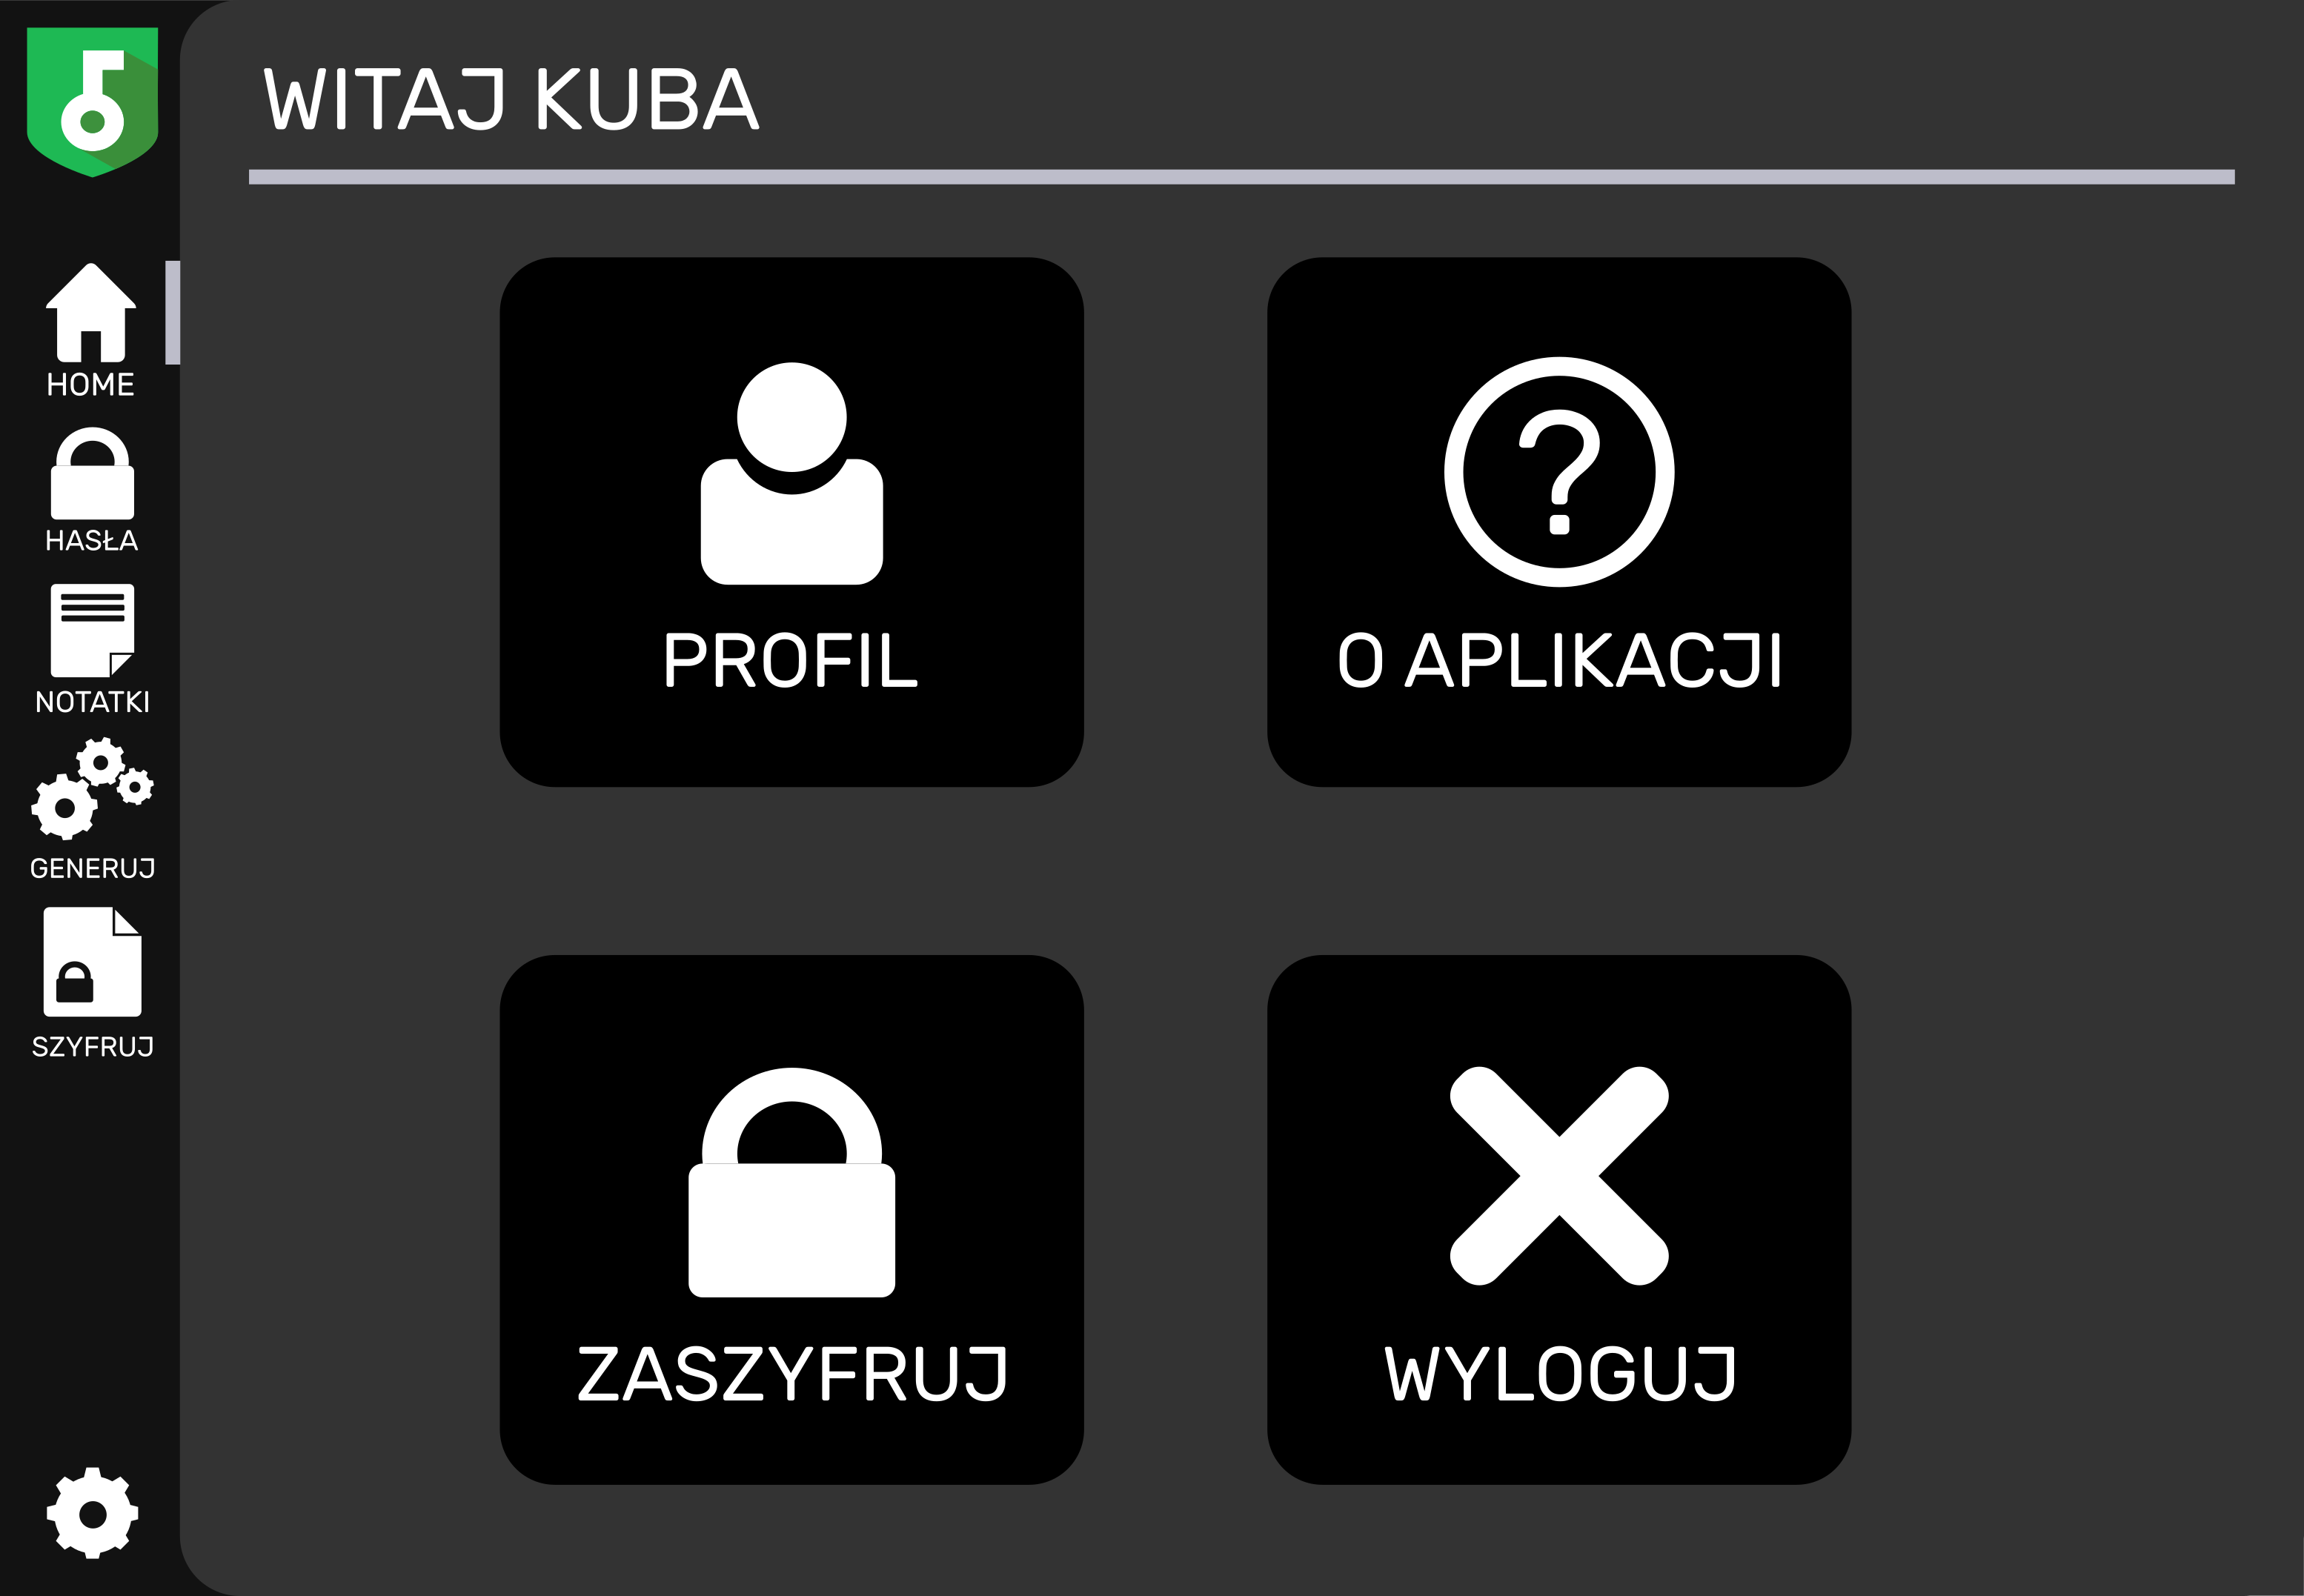
\includegraphics[width=1\textwidth]{img/ekran_po_zalogowaniu.png}
    \caption{Ekran startowy -- po zalogowaniu}
    \label{fig:startPo}
\end{figure}

\newpage

\paragraph{}Kolejna grafika (rys. \ref{fig:rejestracja}.) ukazuje nam ekran, przy pomocy którego możemy zarejestrować się do aplikacji. Po rejestracji przeniesieni zostaniemy do ekranu na rysunku \ref{fig:startPo}.
\begin{figure}[H]
    \centering
    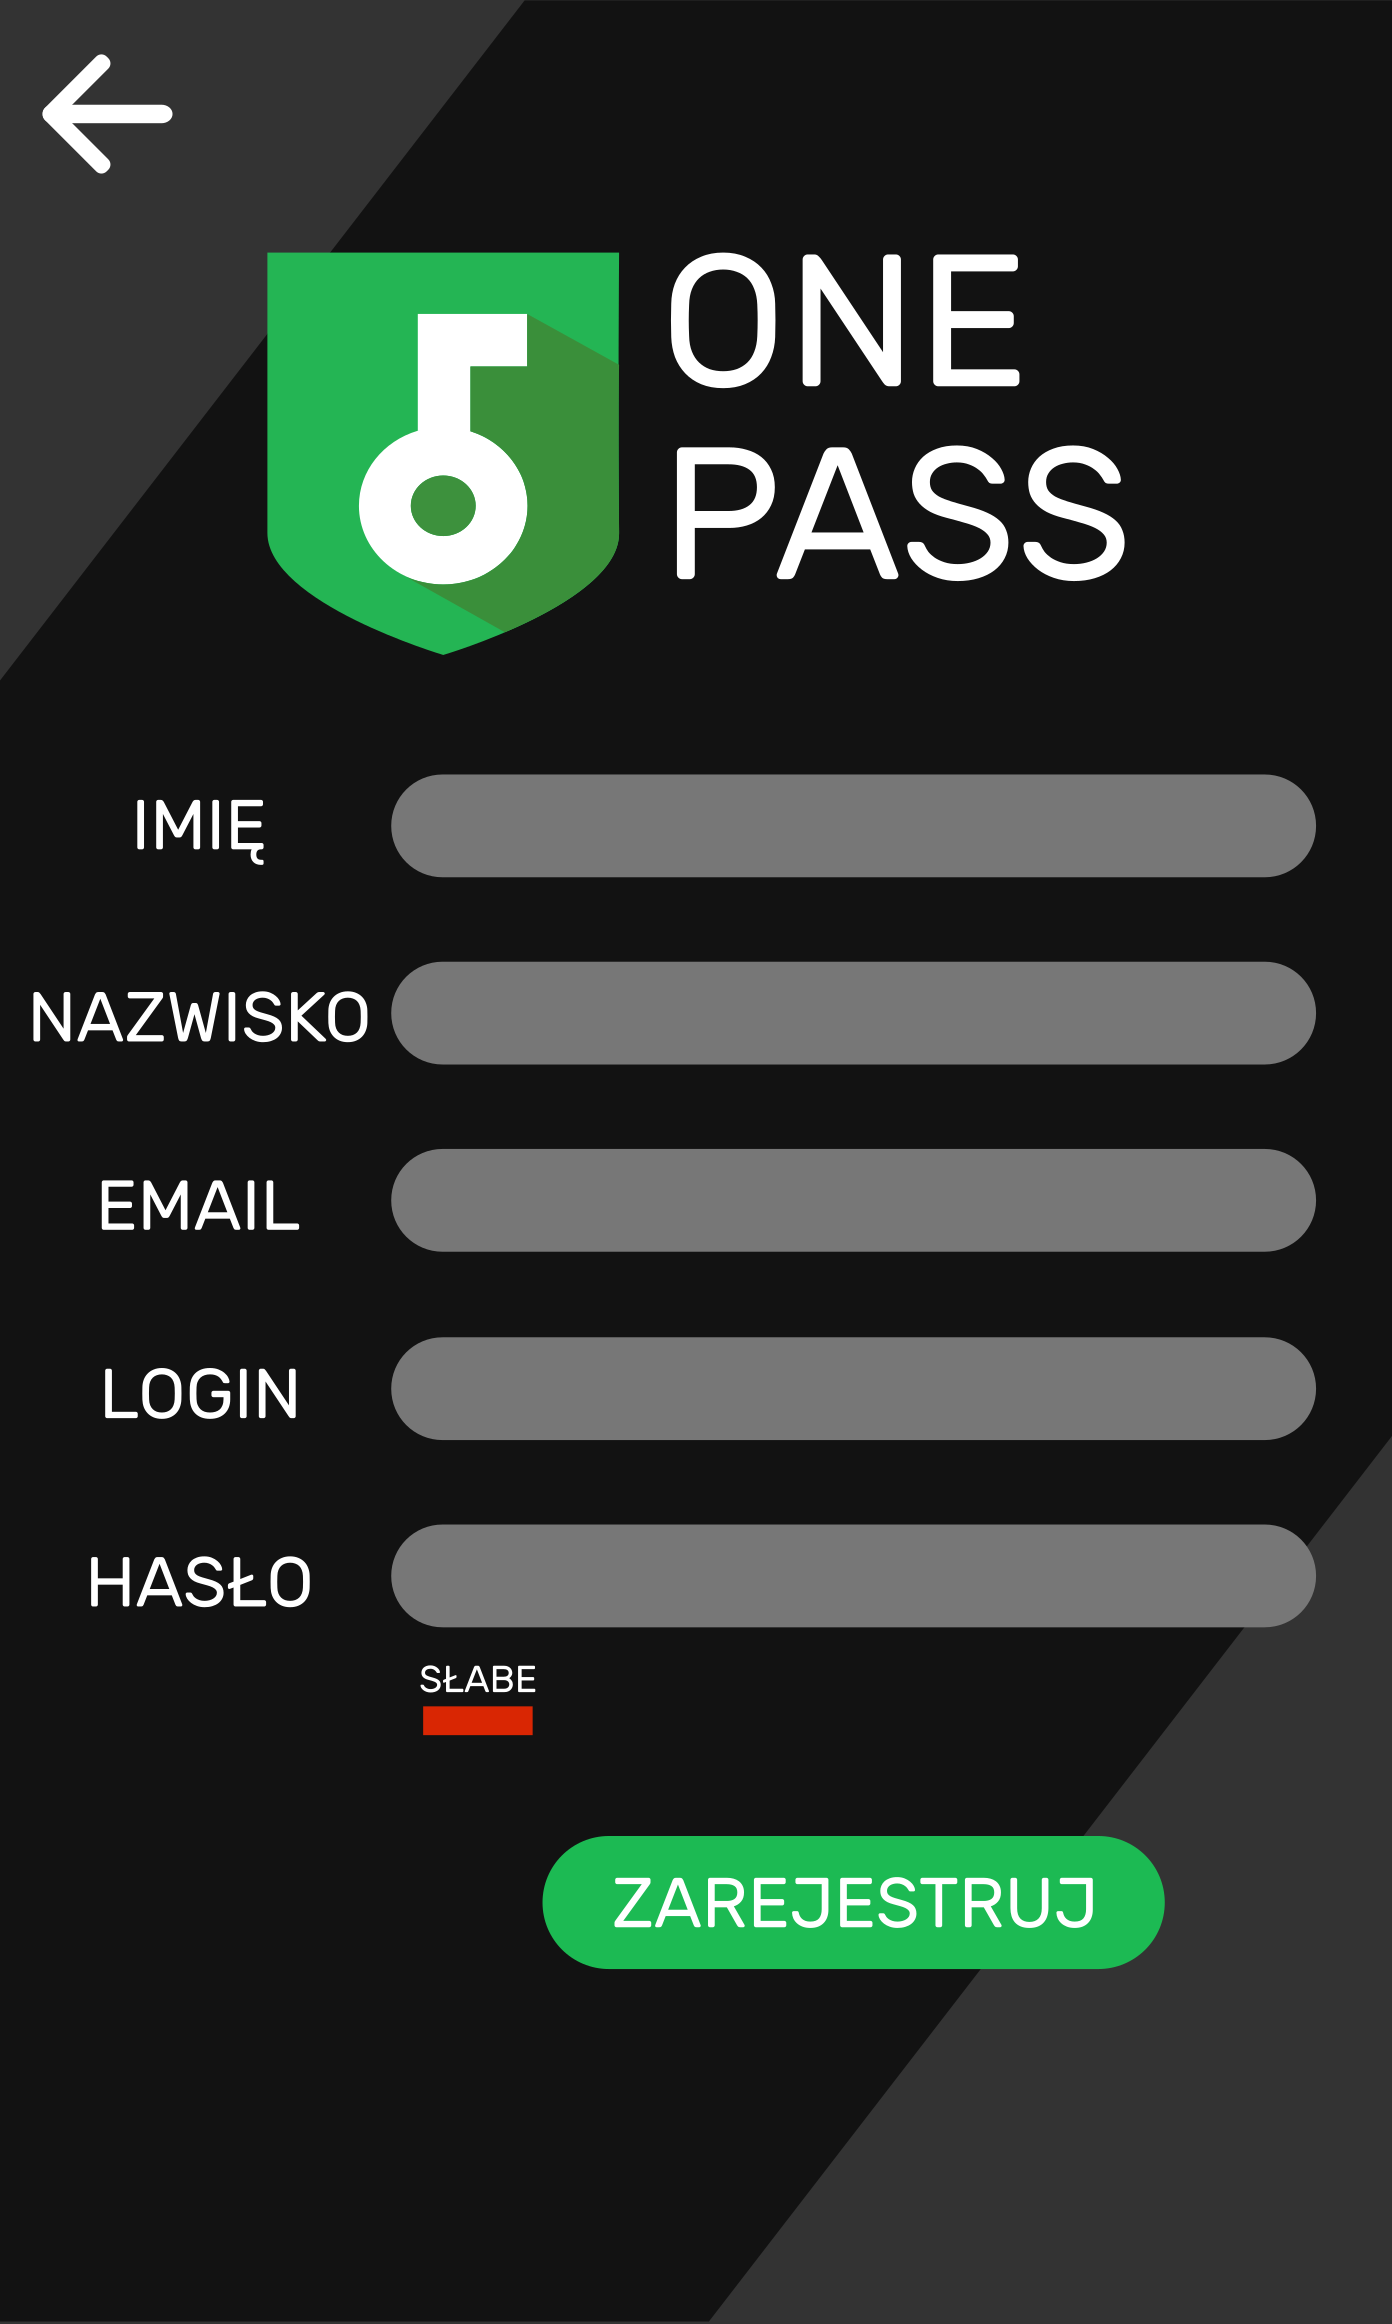
\includegraphics[height=1\textwidth]{img/ekran_rejestracji.png}
    \caption{Ekran rejestracji}
    \label{fig:rejestracja}
\end{figure}

\newpage

\paragraph{}Rysunek \ref{fig:generuj}. prezentuje ekran generowania haseł. Dostęp do tego ekranu nie wymaga zalogowania się do aplikacji.
\begin{figure}[H]
    \centering
    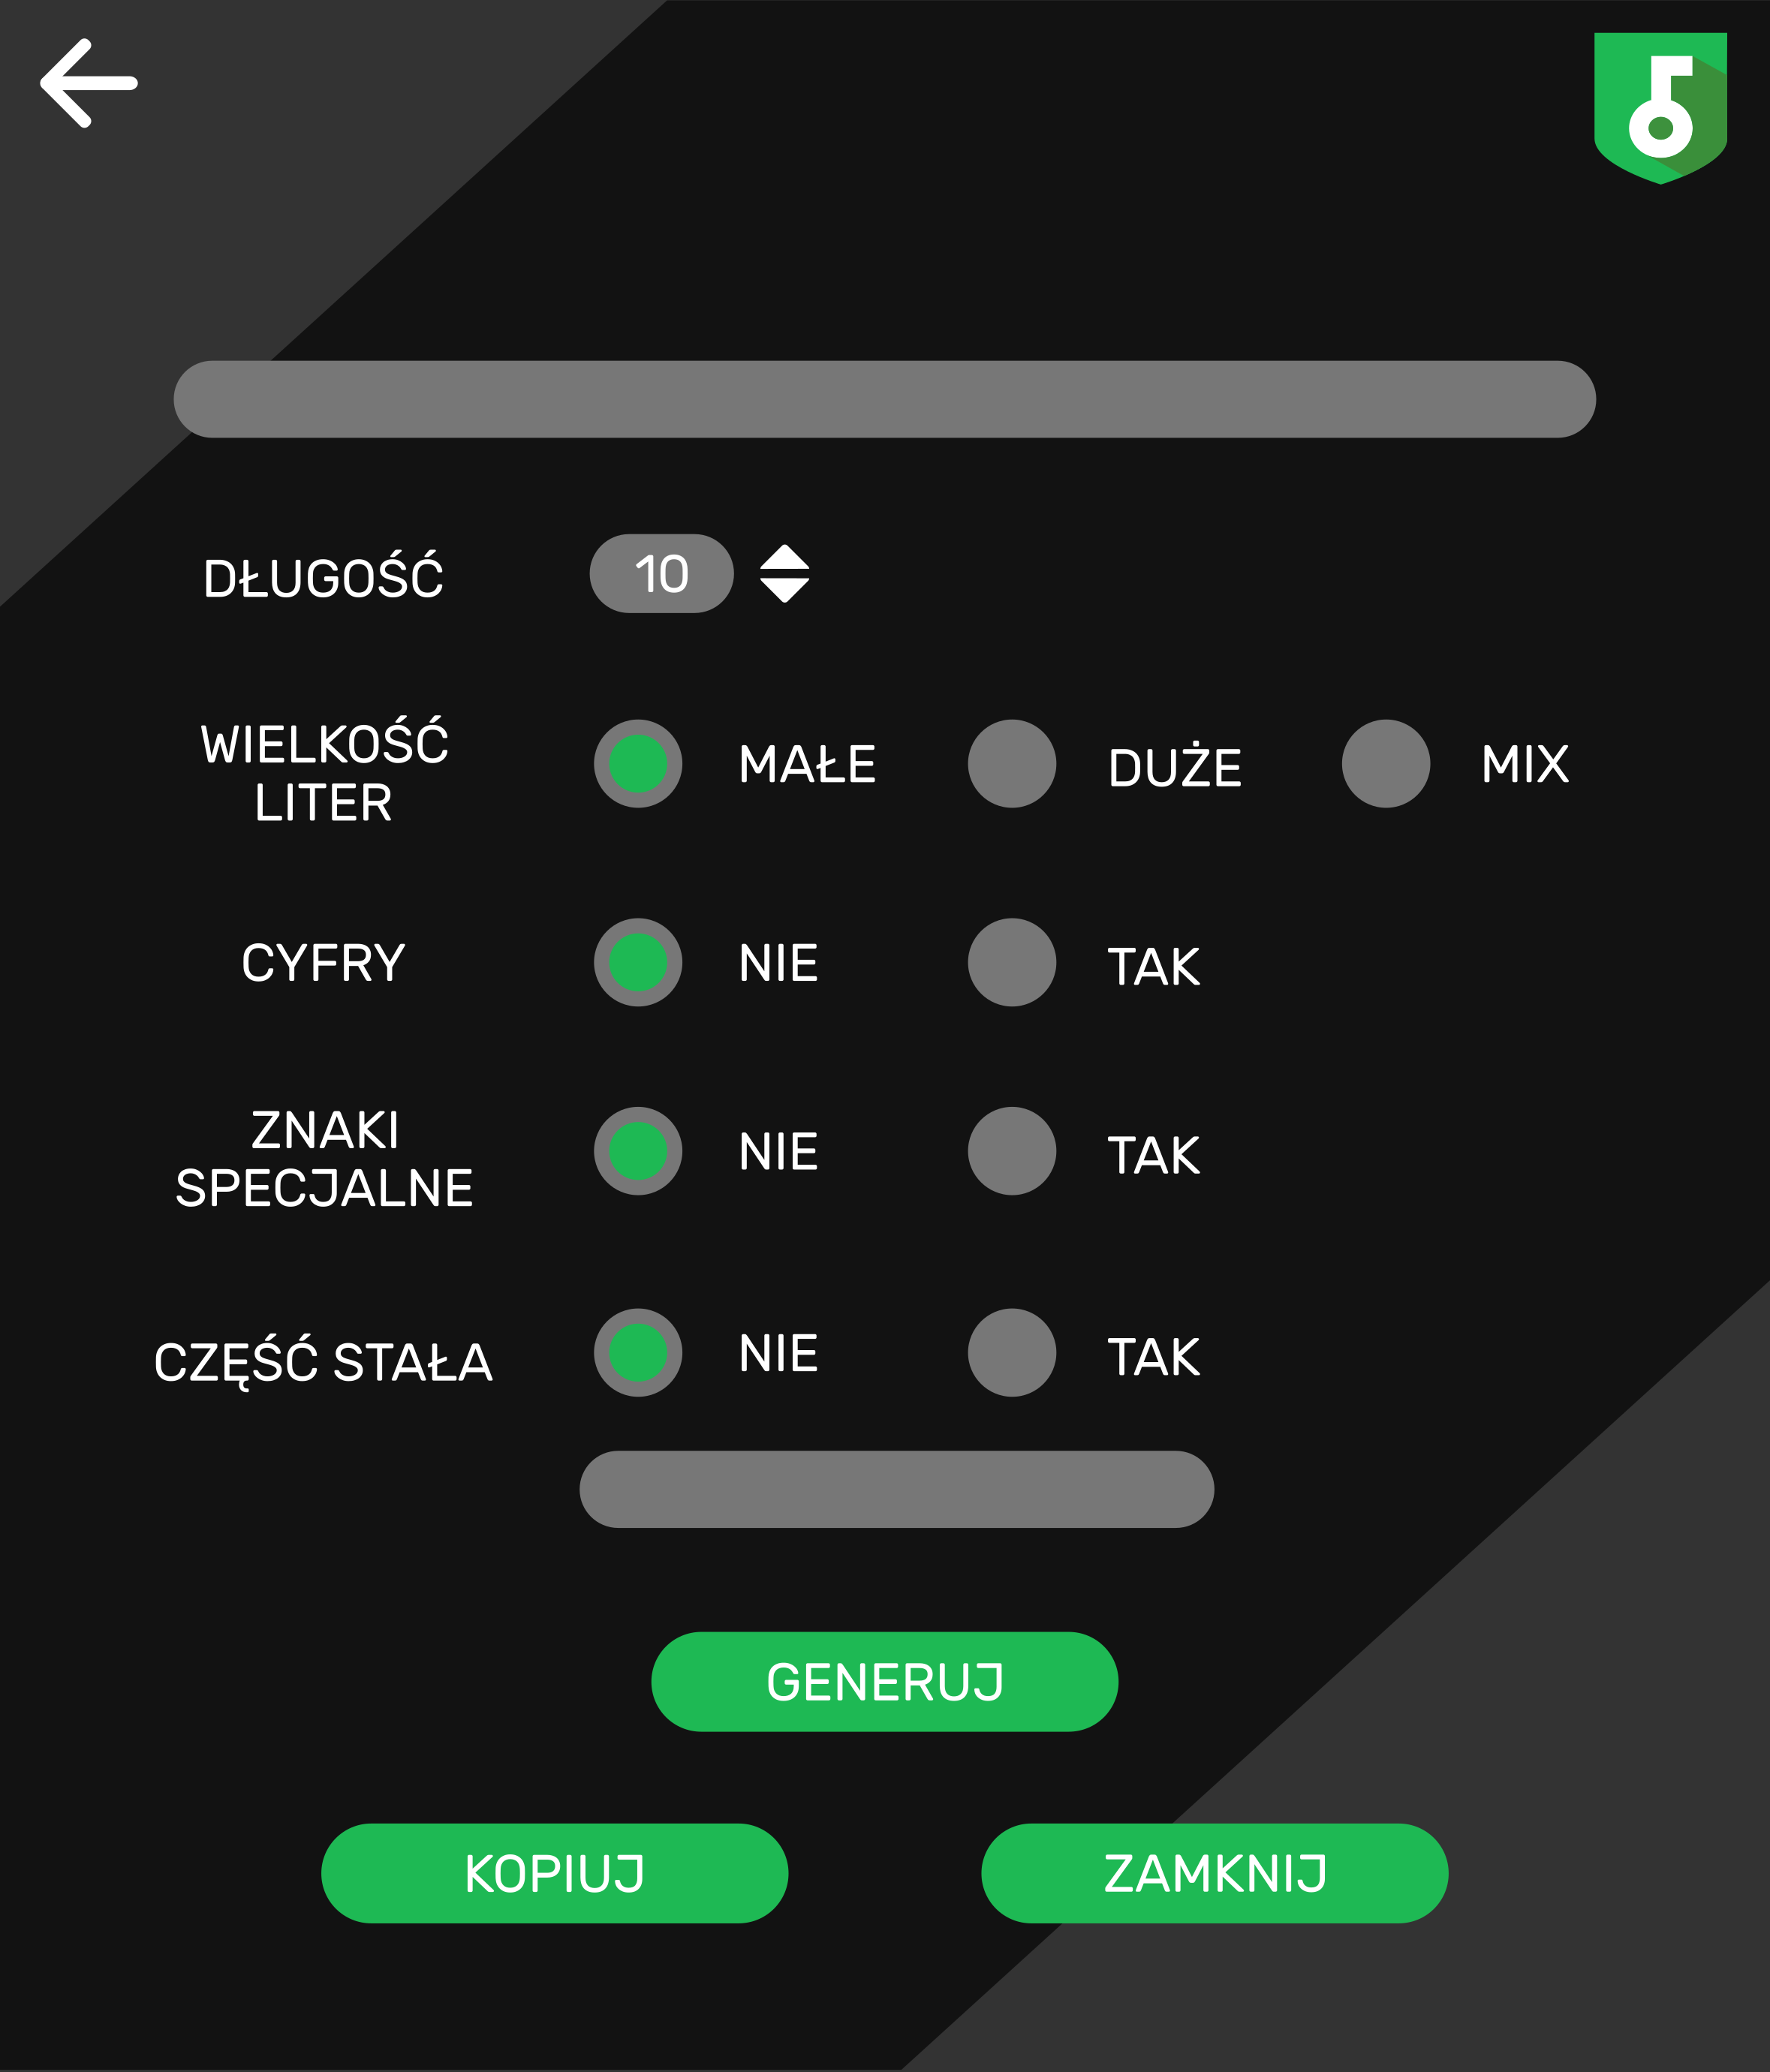
\includegraphics[height=1\textwidth]{img/ekran_generowania.png}
    \caption{Ekran generowania haseł}
    \label{fig:generuj}
\end{figure}

\newpage

\paragraph{}Na ekranie przedstawionym na rysunku \ref{fig:oAplikacj}. zostanie zamieszczona informacja o aplikacaji oraz informacje o autorze. Istnieje możliwość powrotu do ekranu głównego przy pomocy przycisku strzałki lub przez zamknięcie okna.
\begin{figure}[H]
    \centering
    
\includegraphics[height=1\textwidth]{img/ekran_o_aplikacji.png}
    \caption{Ekran o aplikacji}
    \label{fig:oAplikacj}
\end{figure}

\newpage

\paragraph{}Na rysunku \ref{fig:profil}. widzimy ekran informacji o profilu. W tym miejscu po kliknięciu przycisku \textit{Edytuj} mamy możliwość edycji naszego profilu.
\begin{figure}[H]
    \centering
    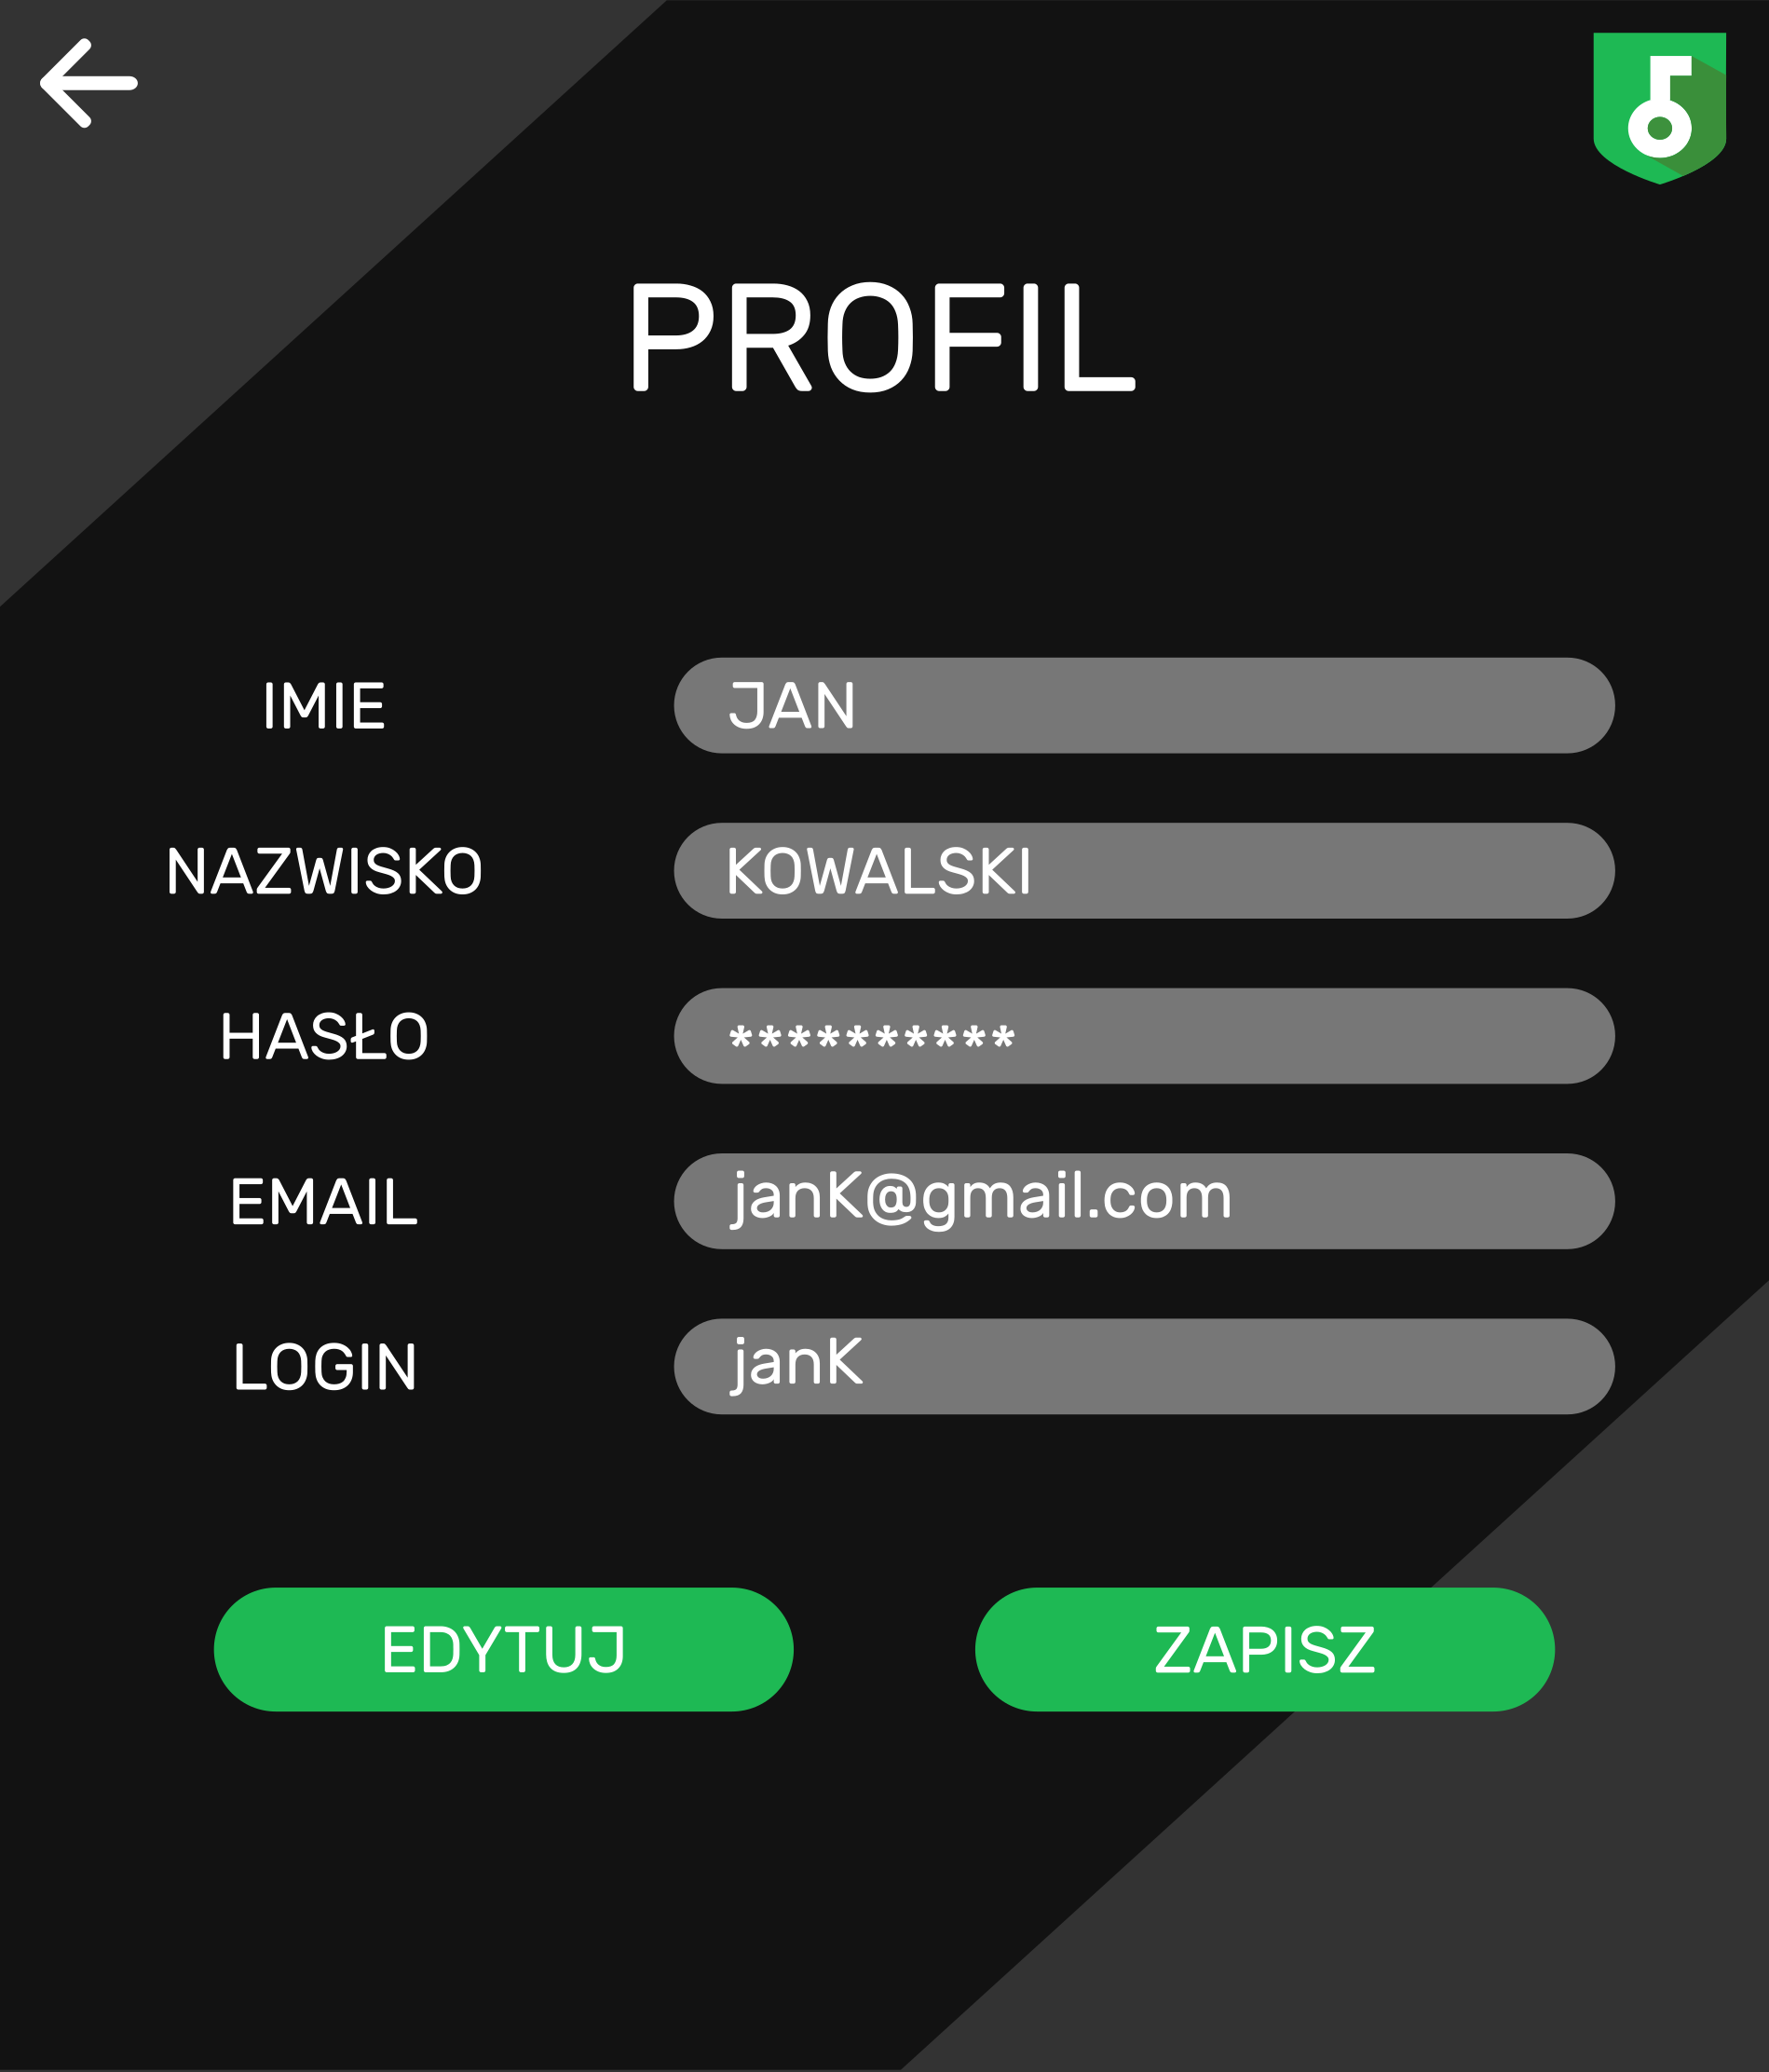
\includegraphics[height=1\textwidth]{img/ekran_profilu.png}
    \caption{Ekran informacji o profilu}
    \label{fig:profil}
\end{figure}

\newpage

\paragraph{}Rysunek \ref{fig:hasła}. przedstawia ekran listy wszystkich haseł zapisanych w aplikacji. Aby dostać się do informacji o obiekcie należy wybrać ikonę, a następnie kliknąć przycisk \textit{Wybierz}. Po kliknięciu przycisku z plusem zostaniemy przeniesieni do ekranu na rysunku \ref{fig:hasłoDodaj}.
\begin{figure}[H]
    \centering
    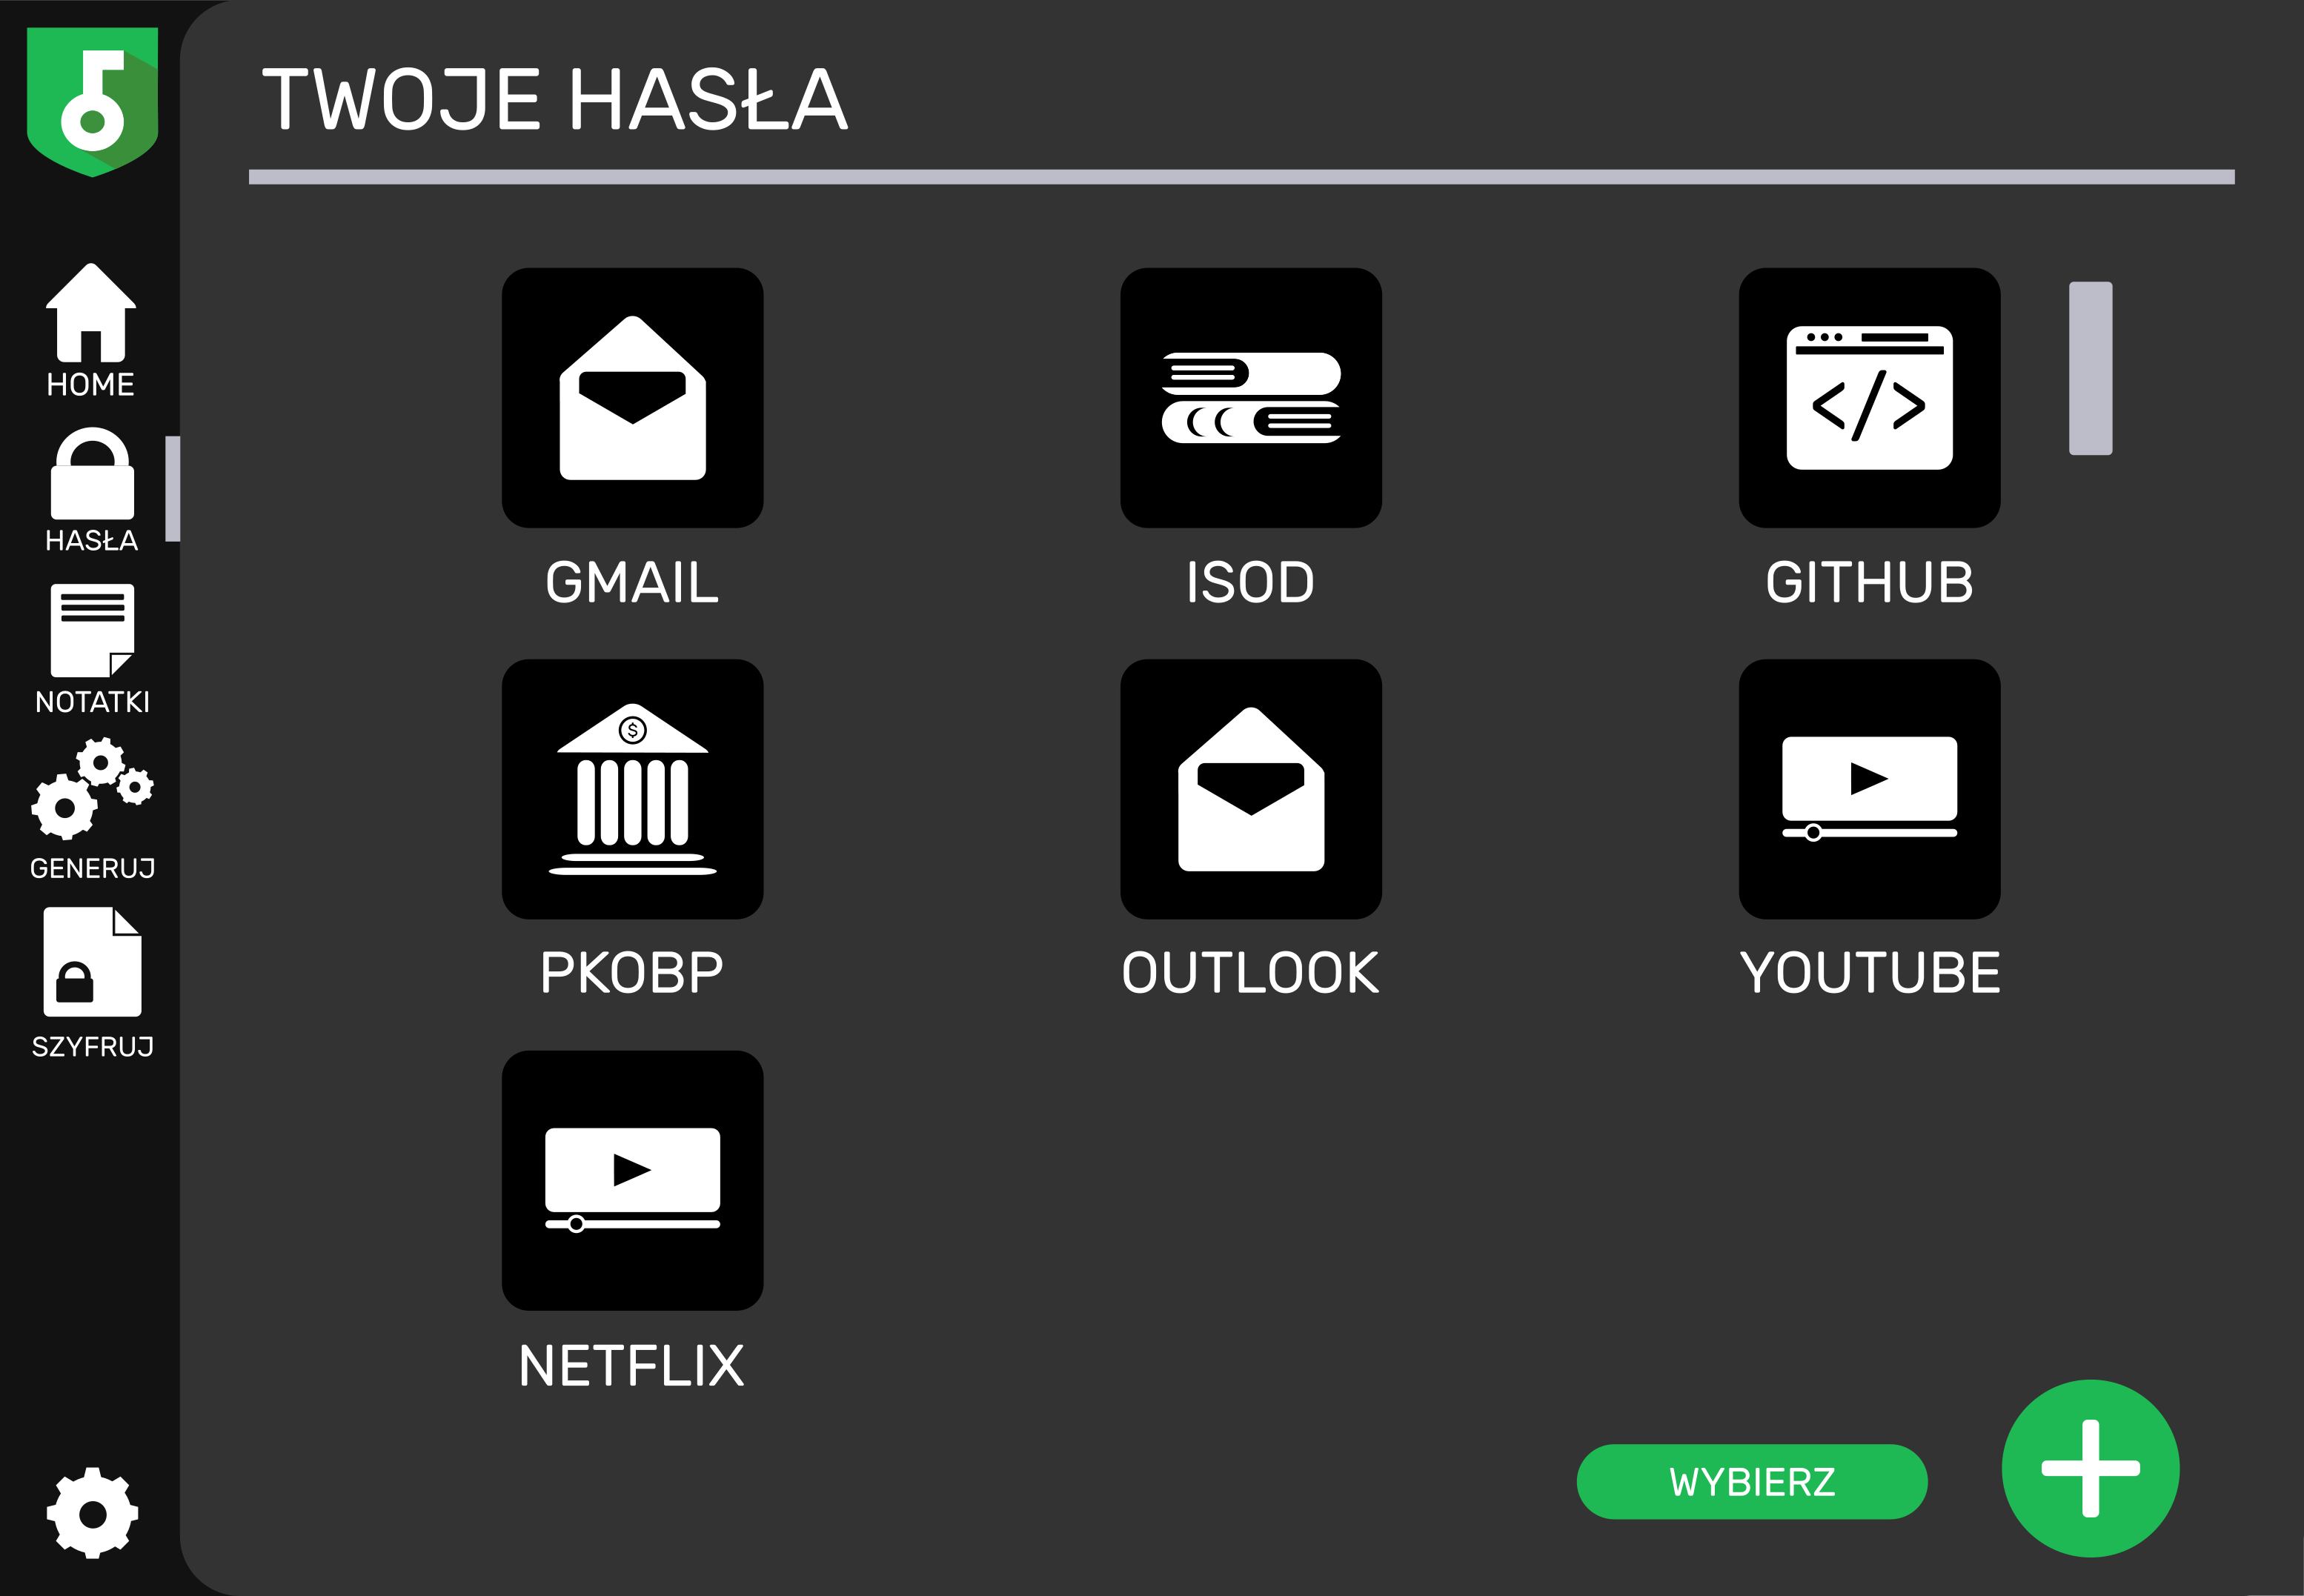
\includegraphics[width=1\textwidth]{img/ekran_hasel.png}
    \caption{Ekran haseł}
    \label{fig:hasła}
\end{figure}

\newpage

\paragraph{}Rysunek \ref{fig:hasłaObiekt}. przedstawia okno opisu obiektu po kliknięciu przycisku \textit{Wybierz} na ekranie z rysunku \ref{fig:hasła}. Na ekranie znajdują się 3 przyciski:
\begin{enumerate}
    \item Kopiuj -- przycisk kopiujący do schowka hasło.
    \item Edytuj -- przycisk umożliwiający edycję obiektu.
    \item Pokaż -- przycisk ujawniające niewidoczne domyślnie hasło.
\end{enumerate}
Dodatkowo w rogu znajduje się przycisk gwiazdki. Gdy jest "zaświecony" obiekt w liście będzie znajdował się na początku.
\begin{figure}[H]
    \centering
    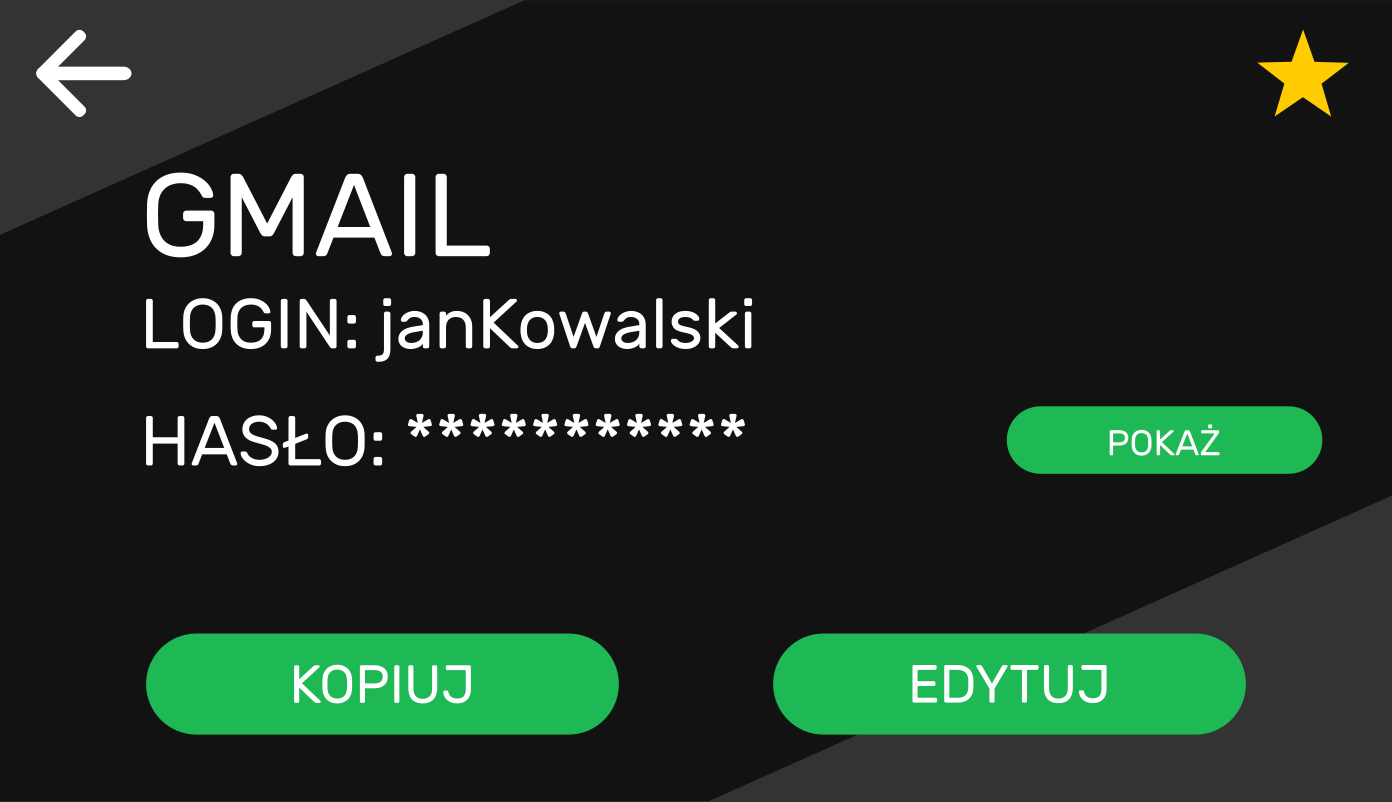
\includegraphics[width=1\textwidth]{img/ekran_obiektu.png}
    \caption{Ekran obiektu}
    \label{fig:hasłaObiekt}
\end{figure}

\newpage

\paragraph{}Na rysunku \ref{fig:hasłoDodaj}. widzimy ekran dodawania nowego obiektu do listy haseł. Przy wyborze kategorii mamy możliwość wyboru ze zbioru kilku kategorii zaprogramowanych. Kategorie definują jaką ikonę otrzyma obiekt w liście haseł.
\begin{figure}[H]
    \centering
    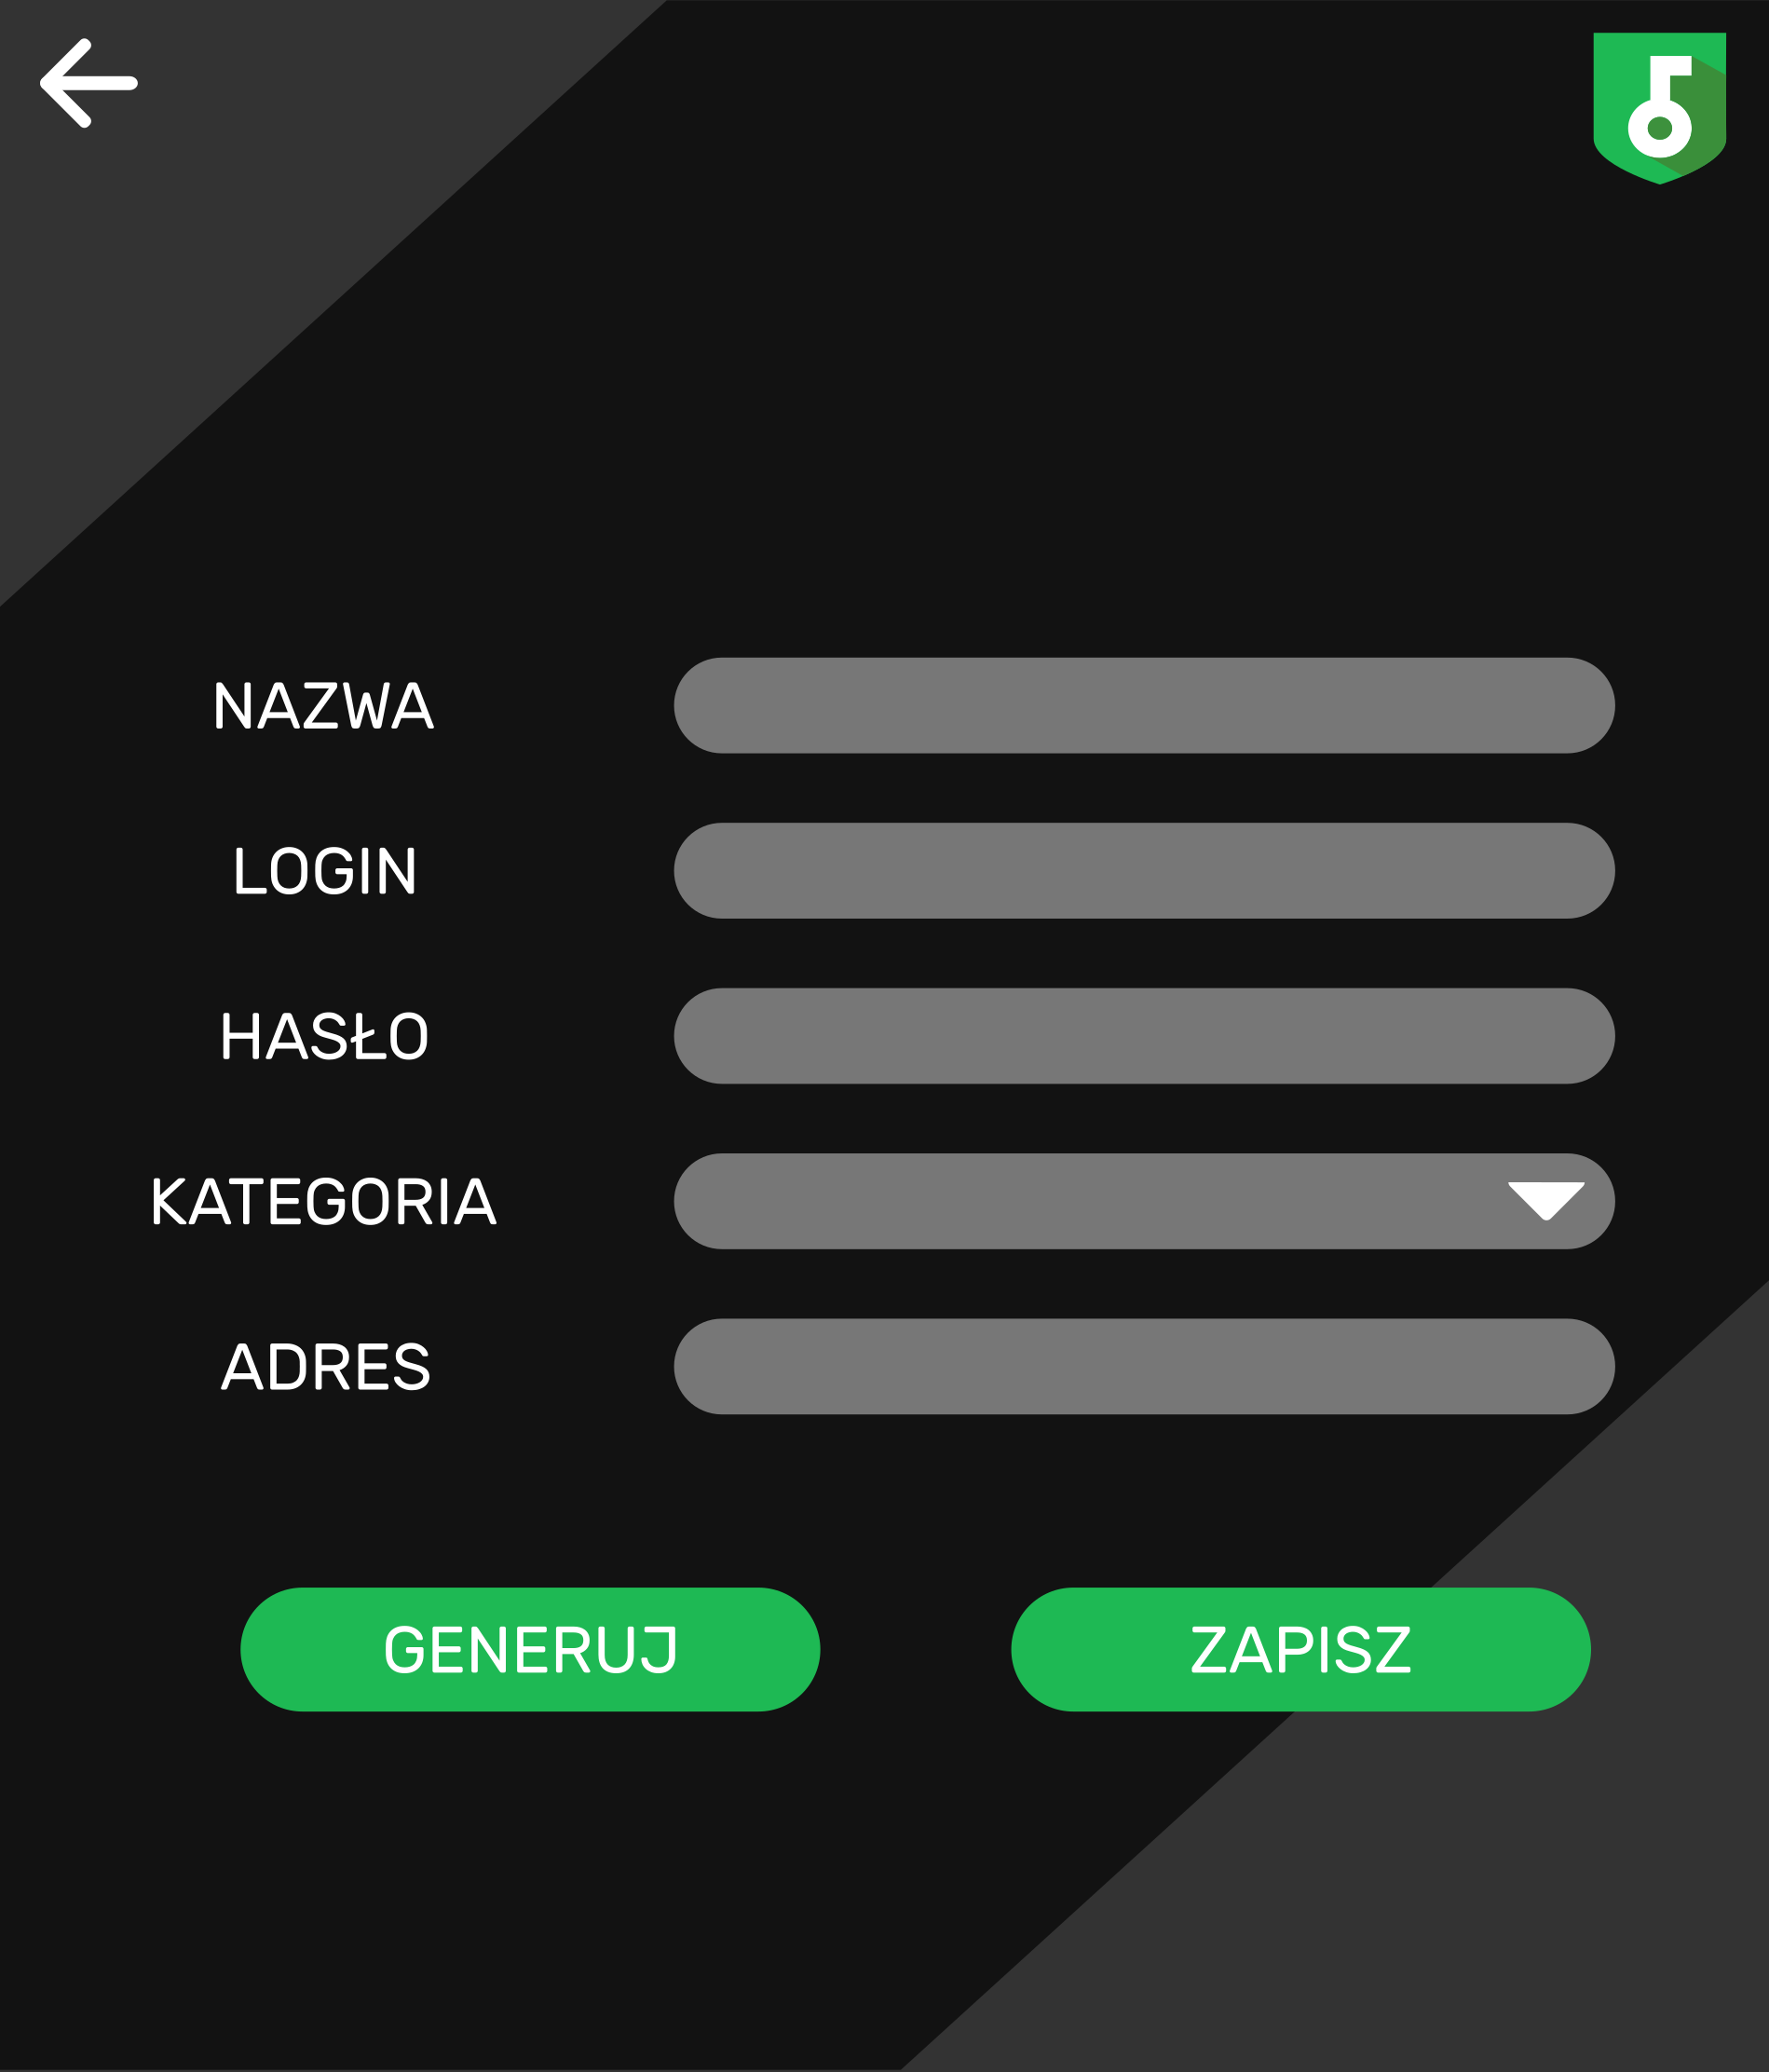
\includegraphics[height=1\textwidth]{img/ekran_dodawania_hasla.png}
    \caption{Ekran dodawania obiektu}
    \label{fig:hasłoDodaj}
\end{figure}

\newpage

\paragraph{}Rysunek \ref{fig:notatki} przedstawia listę zaszyfrowanych notatek. Po wyborze ikony i kliknięciu \textit{Edytuj} przeniesieni zostaniemy do ekranu edycji notatek przedstawionym na rysunku \ref{fig:notatkiNowe}.
\begin{figure}[H]
    \centering
    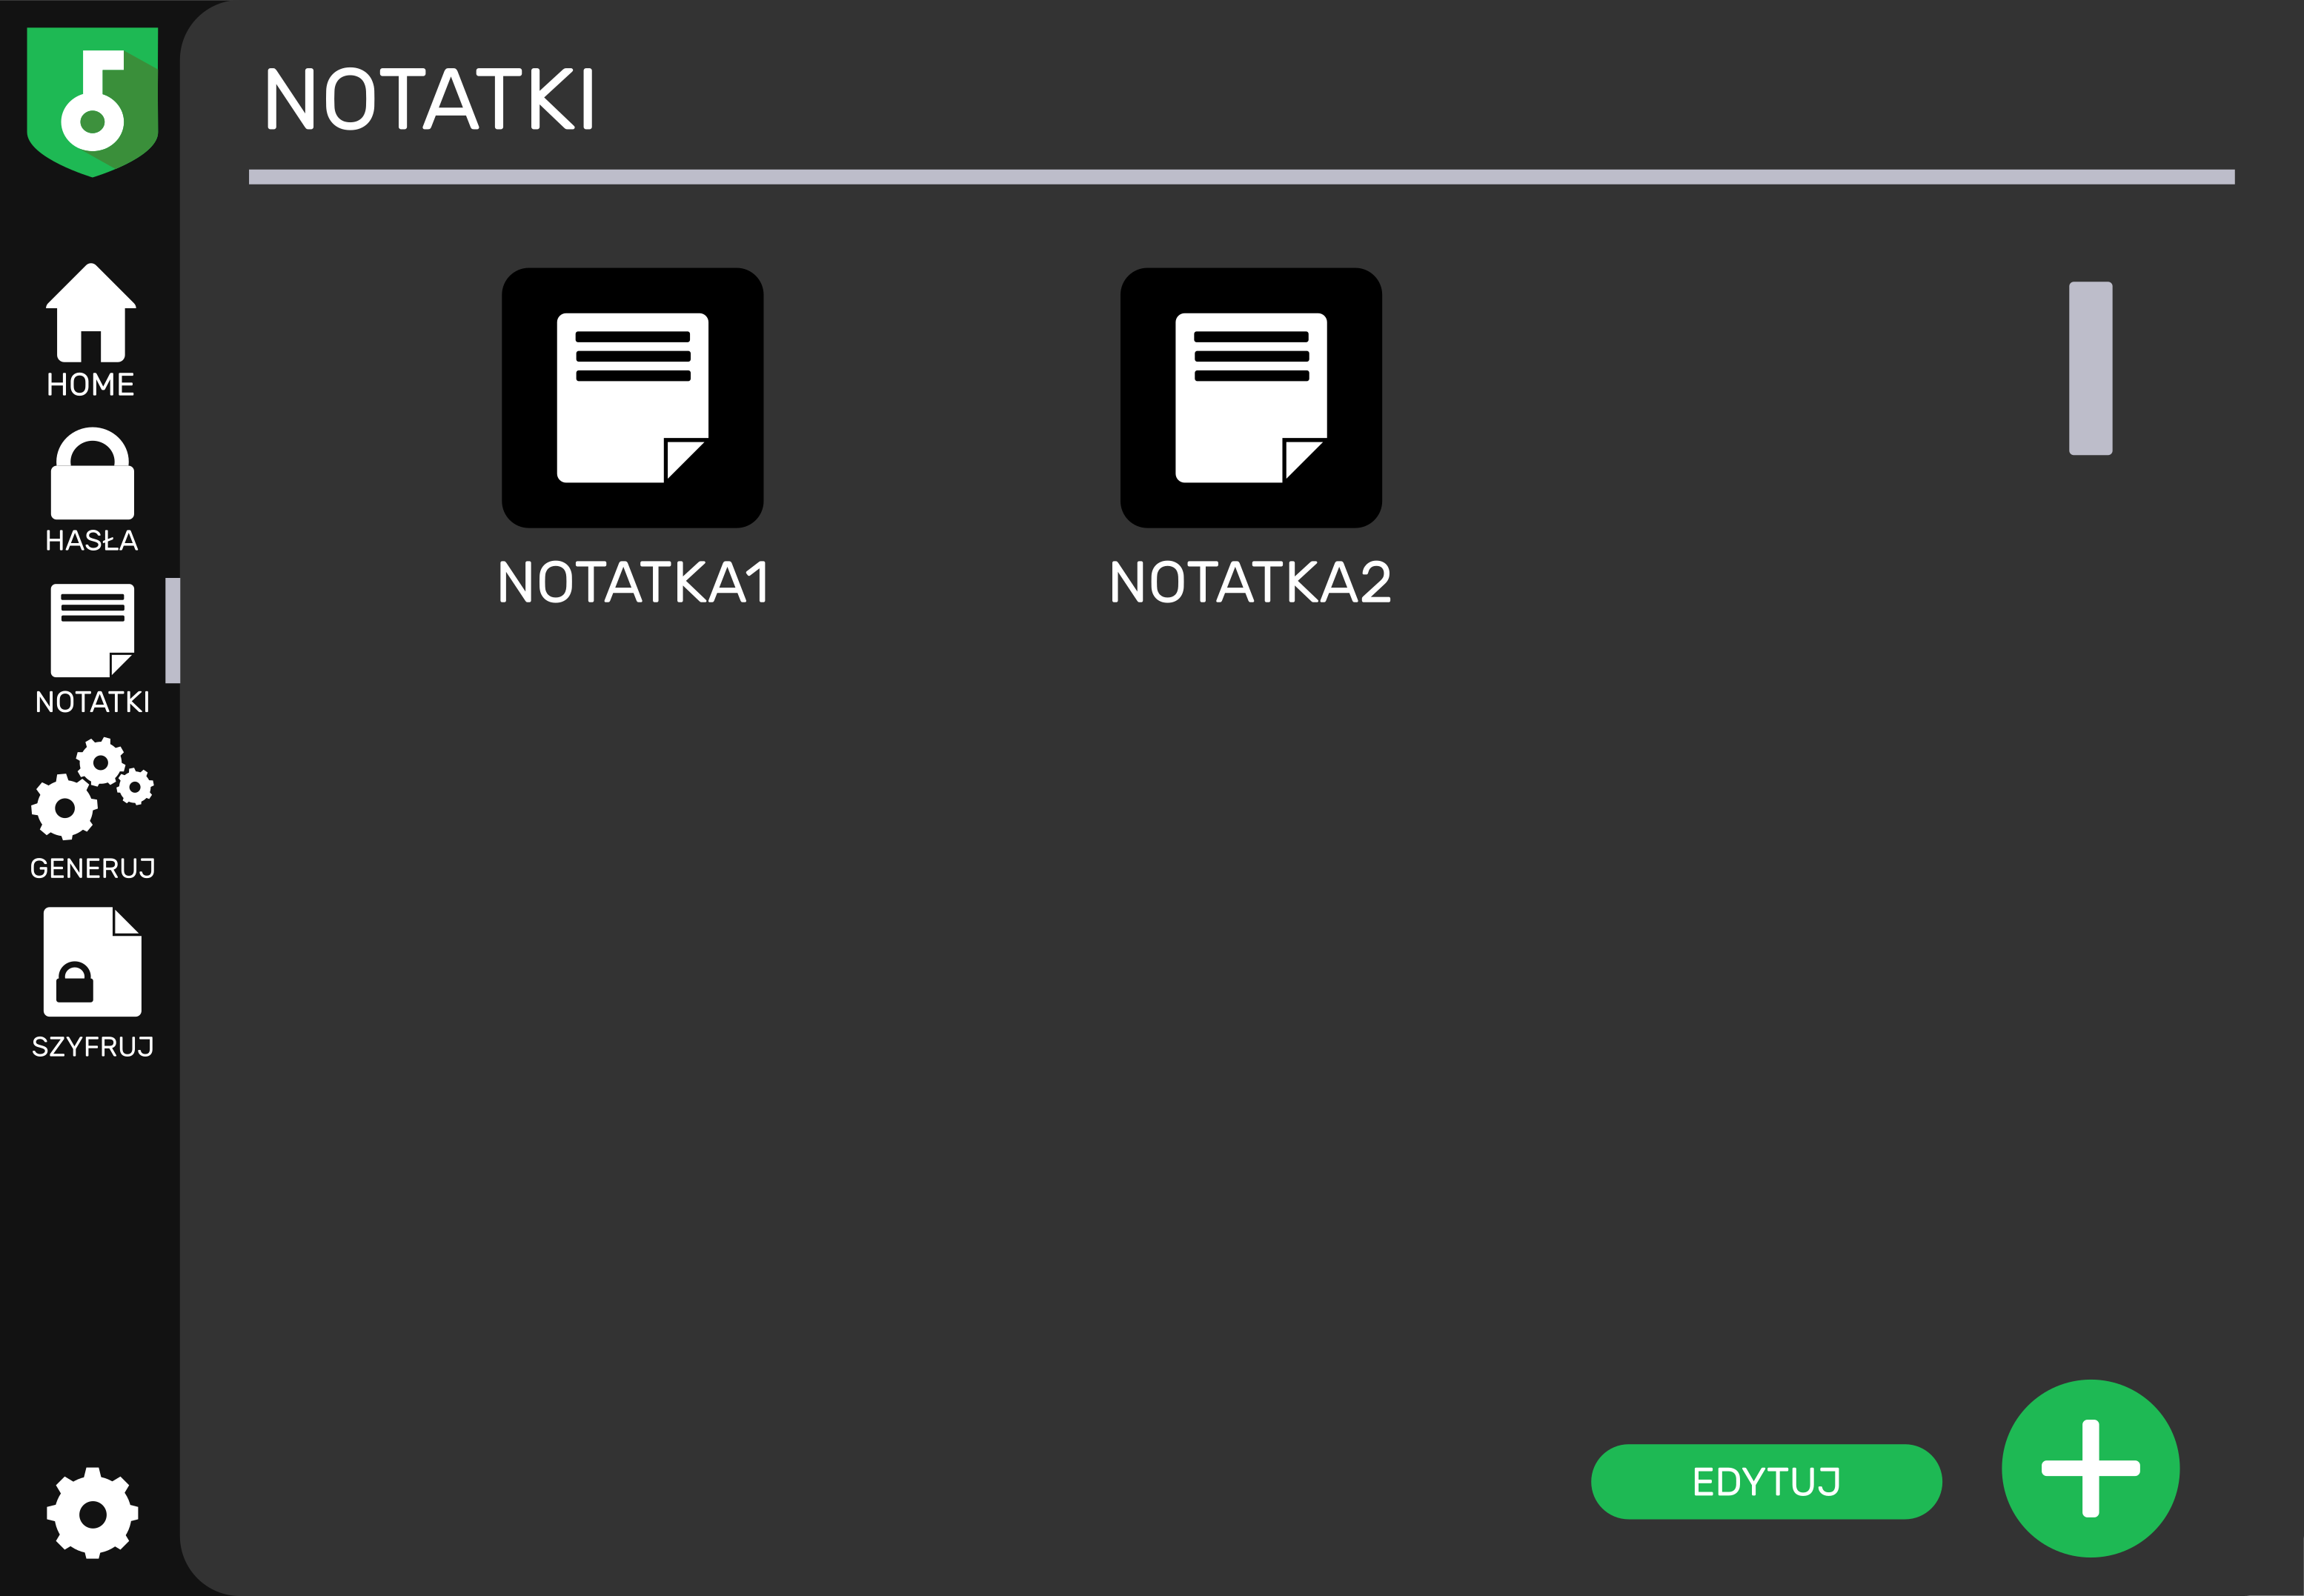
\includegraphics[width=1\textwidth]{img/ekran_notatek.png}
    \caption{Ekran listy notatek}
    \label{fig:notatki}
\end{figure}

\newpage

\paragraph{}Rysunek \ref{fig:notatkiNowe}. prezentuje ekran dodawania lub edycji notatek. W tym miejscu można usunąć istniejącą już notatkę.
\begin{figure}[H]
    \centering
    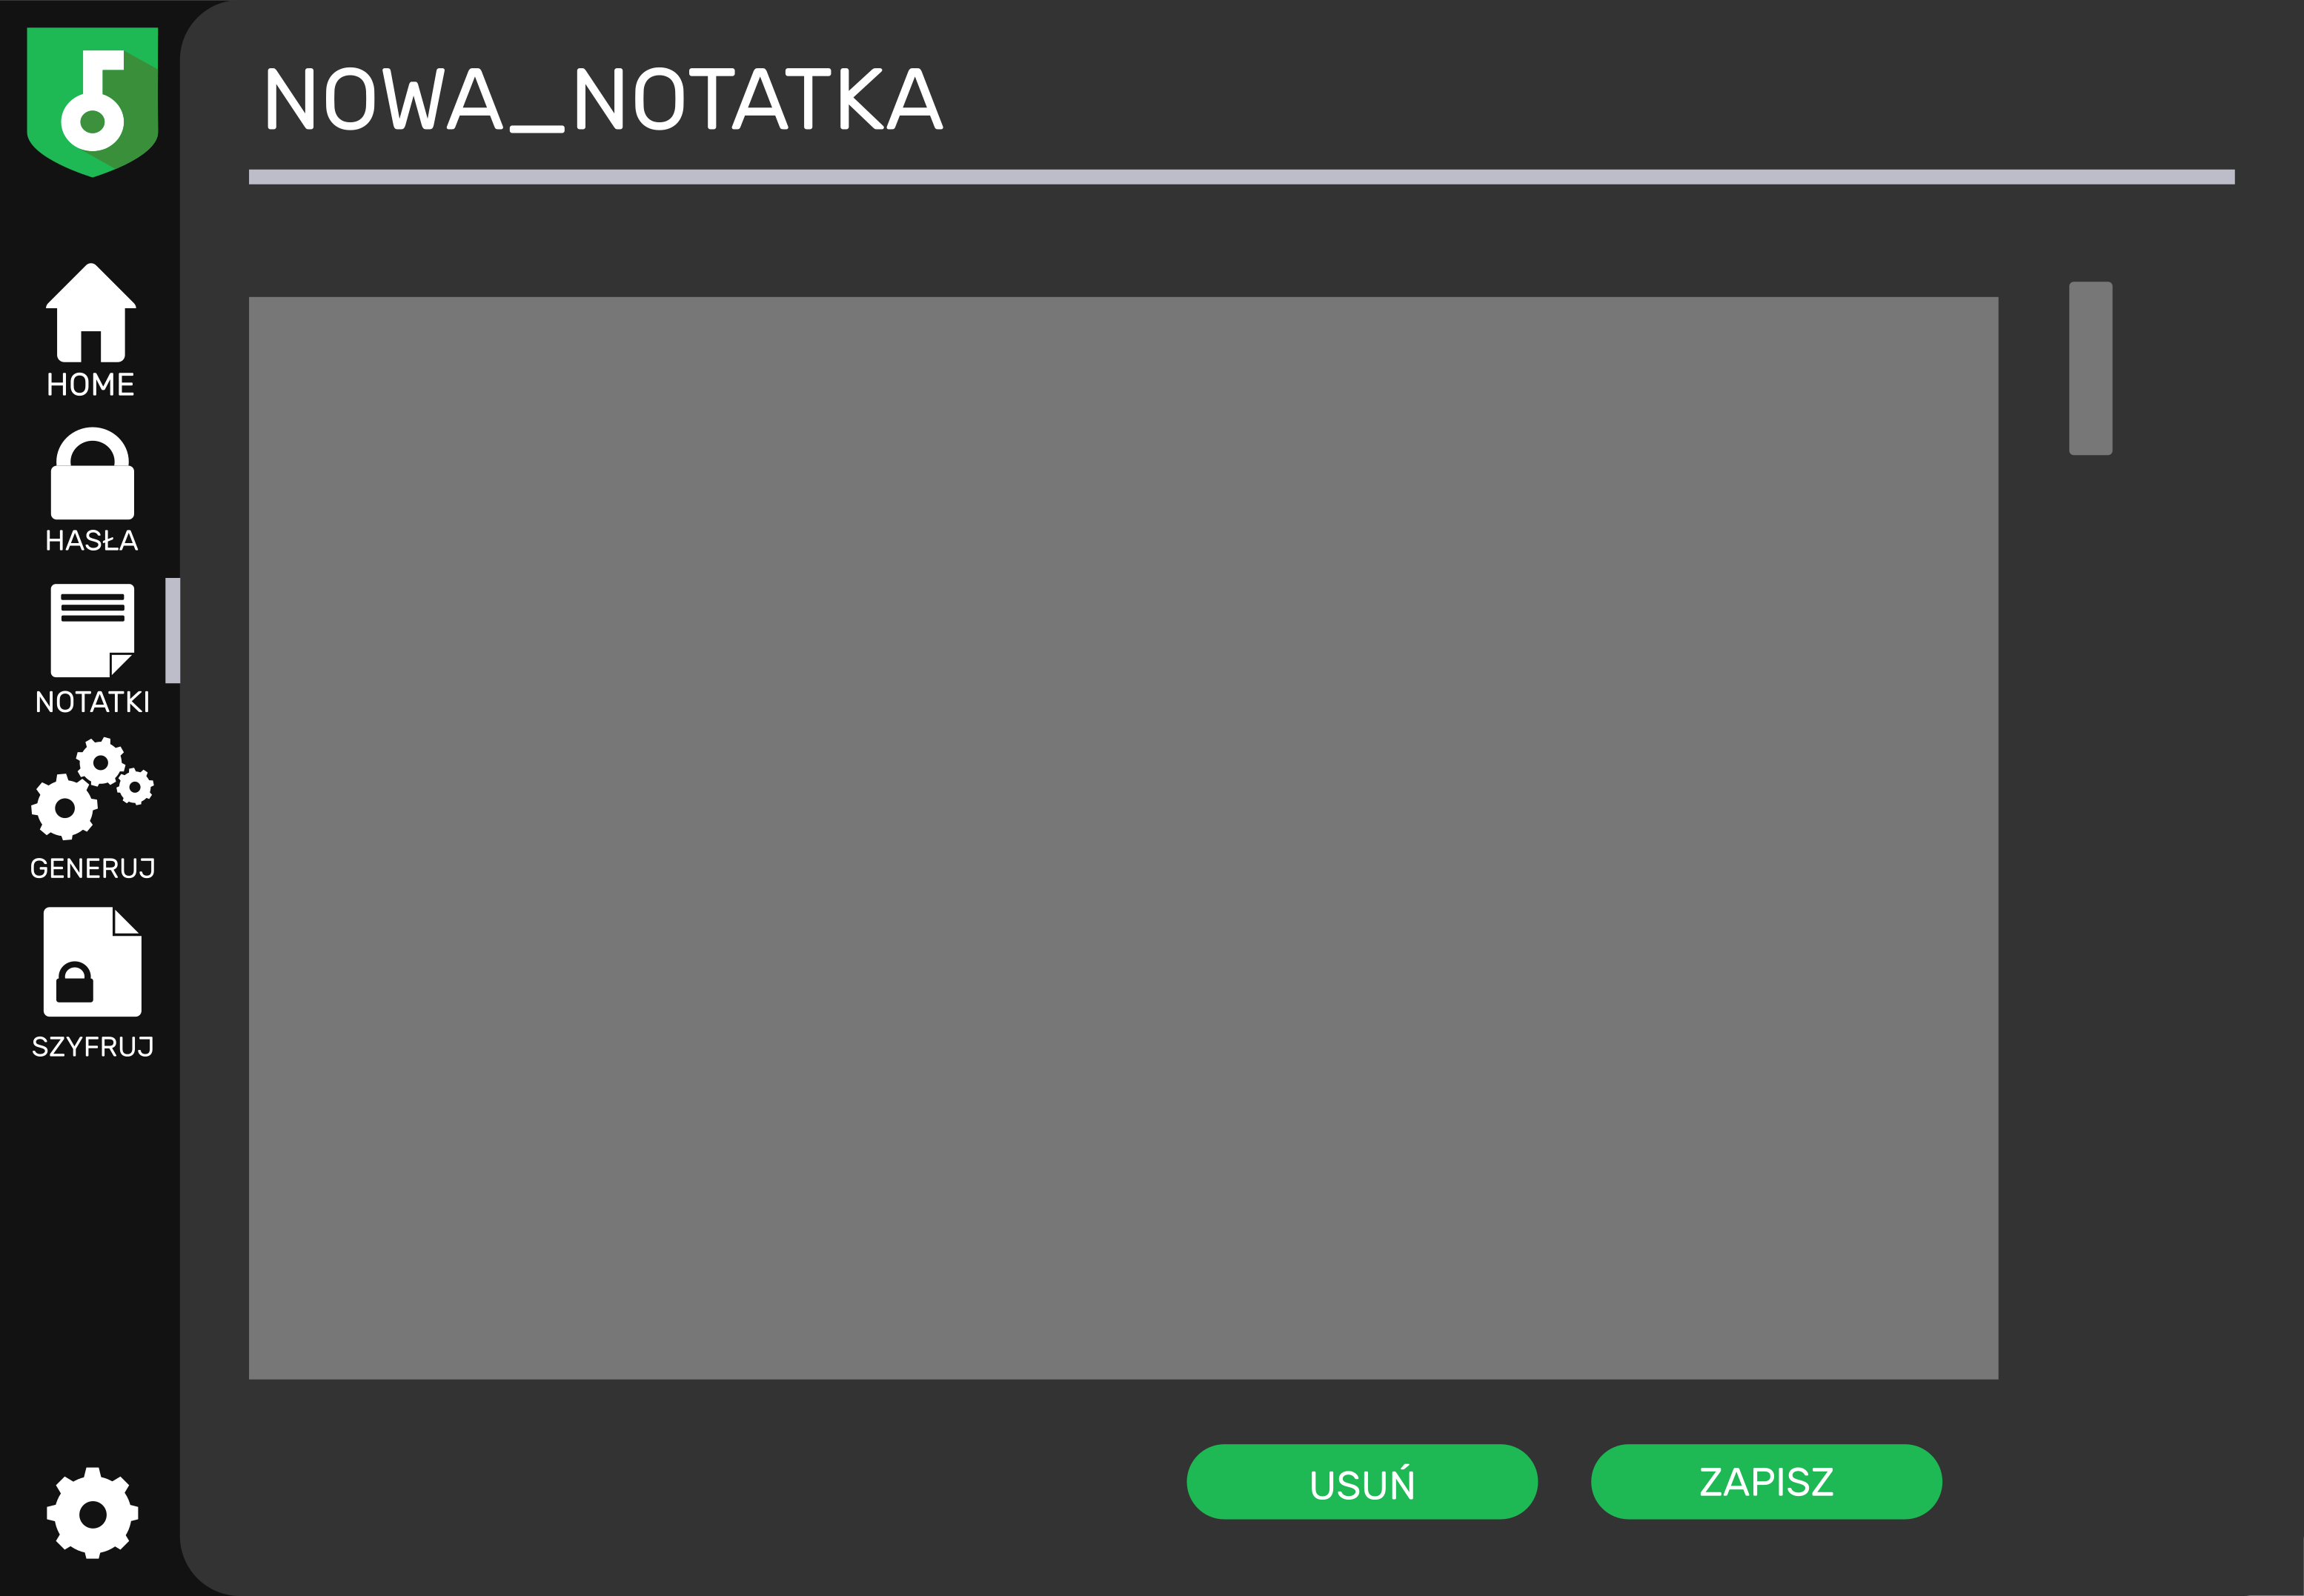
\includegraphics[width=1\textwidth]{img/ekran_notatek_nowa.png}
    \caption{Ekran dodawania lub edycji notatek}
    \label{fig:notatkiNowe}
\end{figure}

\newpage

\paragraph{}Na ekranie przedstawionym na rysunku \ref{fig:szyfrowanie}. można zaszyfrować podany przez siebie plik lub rozszyfrować plik wcześniej zaszyfrowany.
\begin{figure}[H]
    \centering
    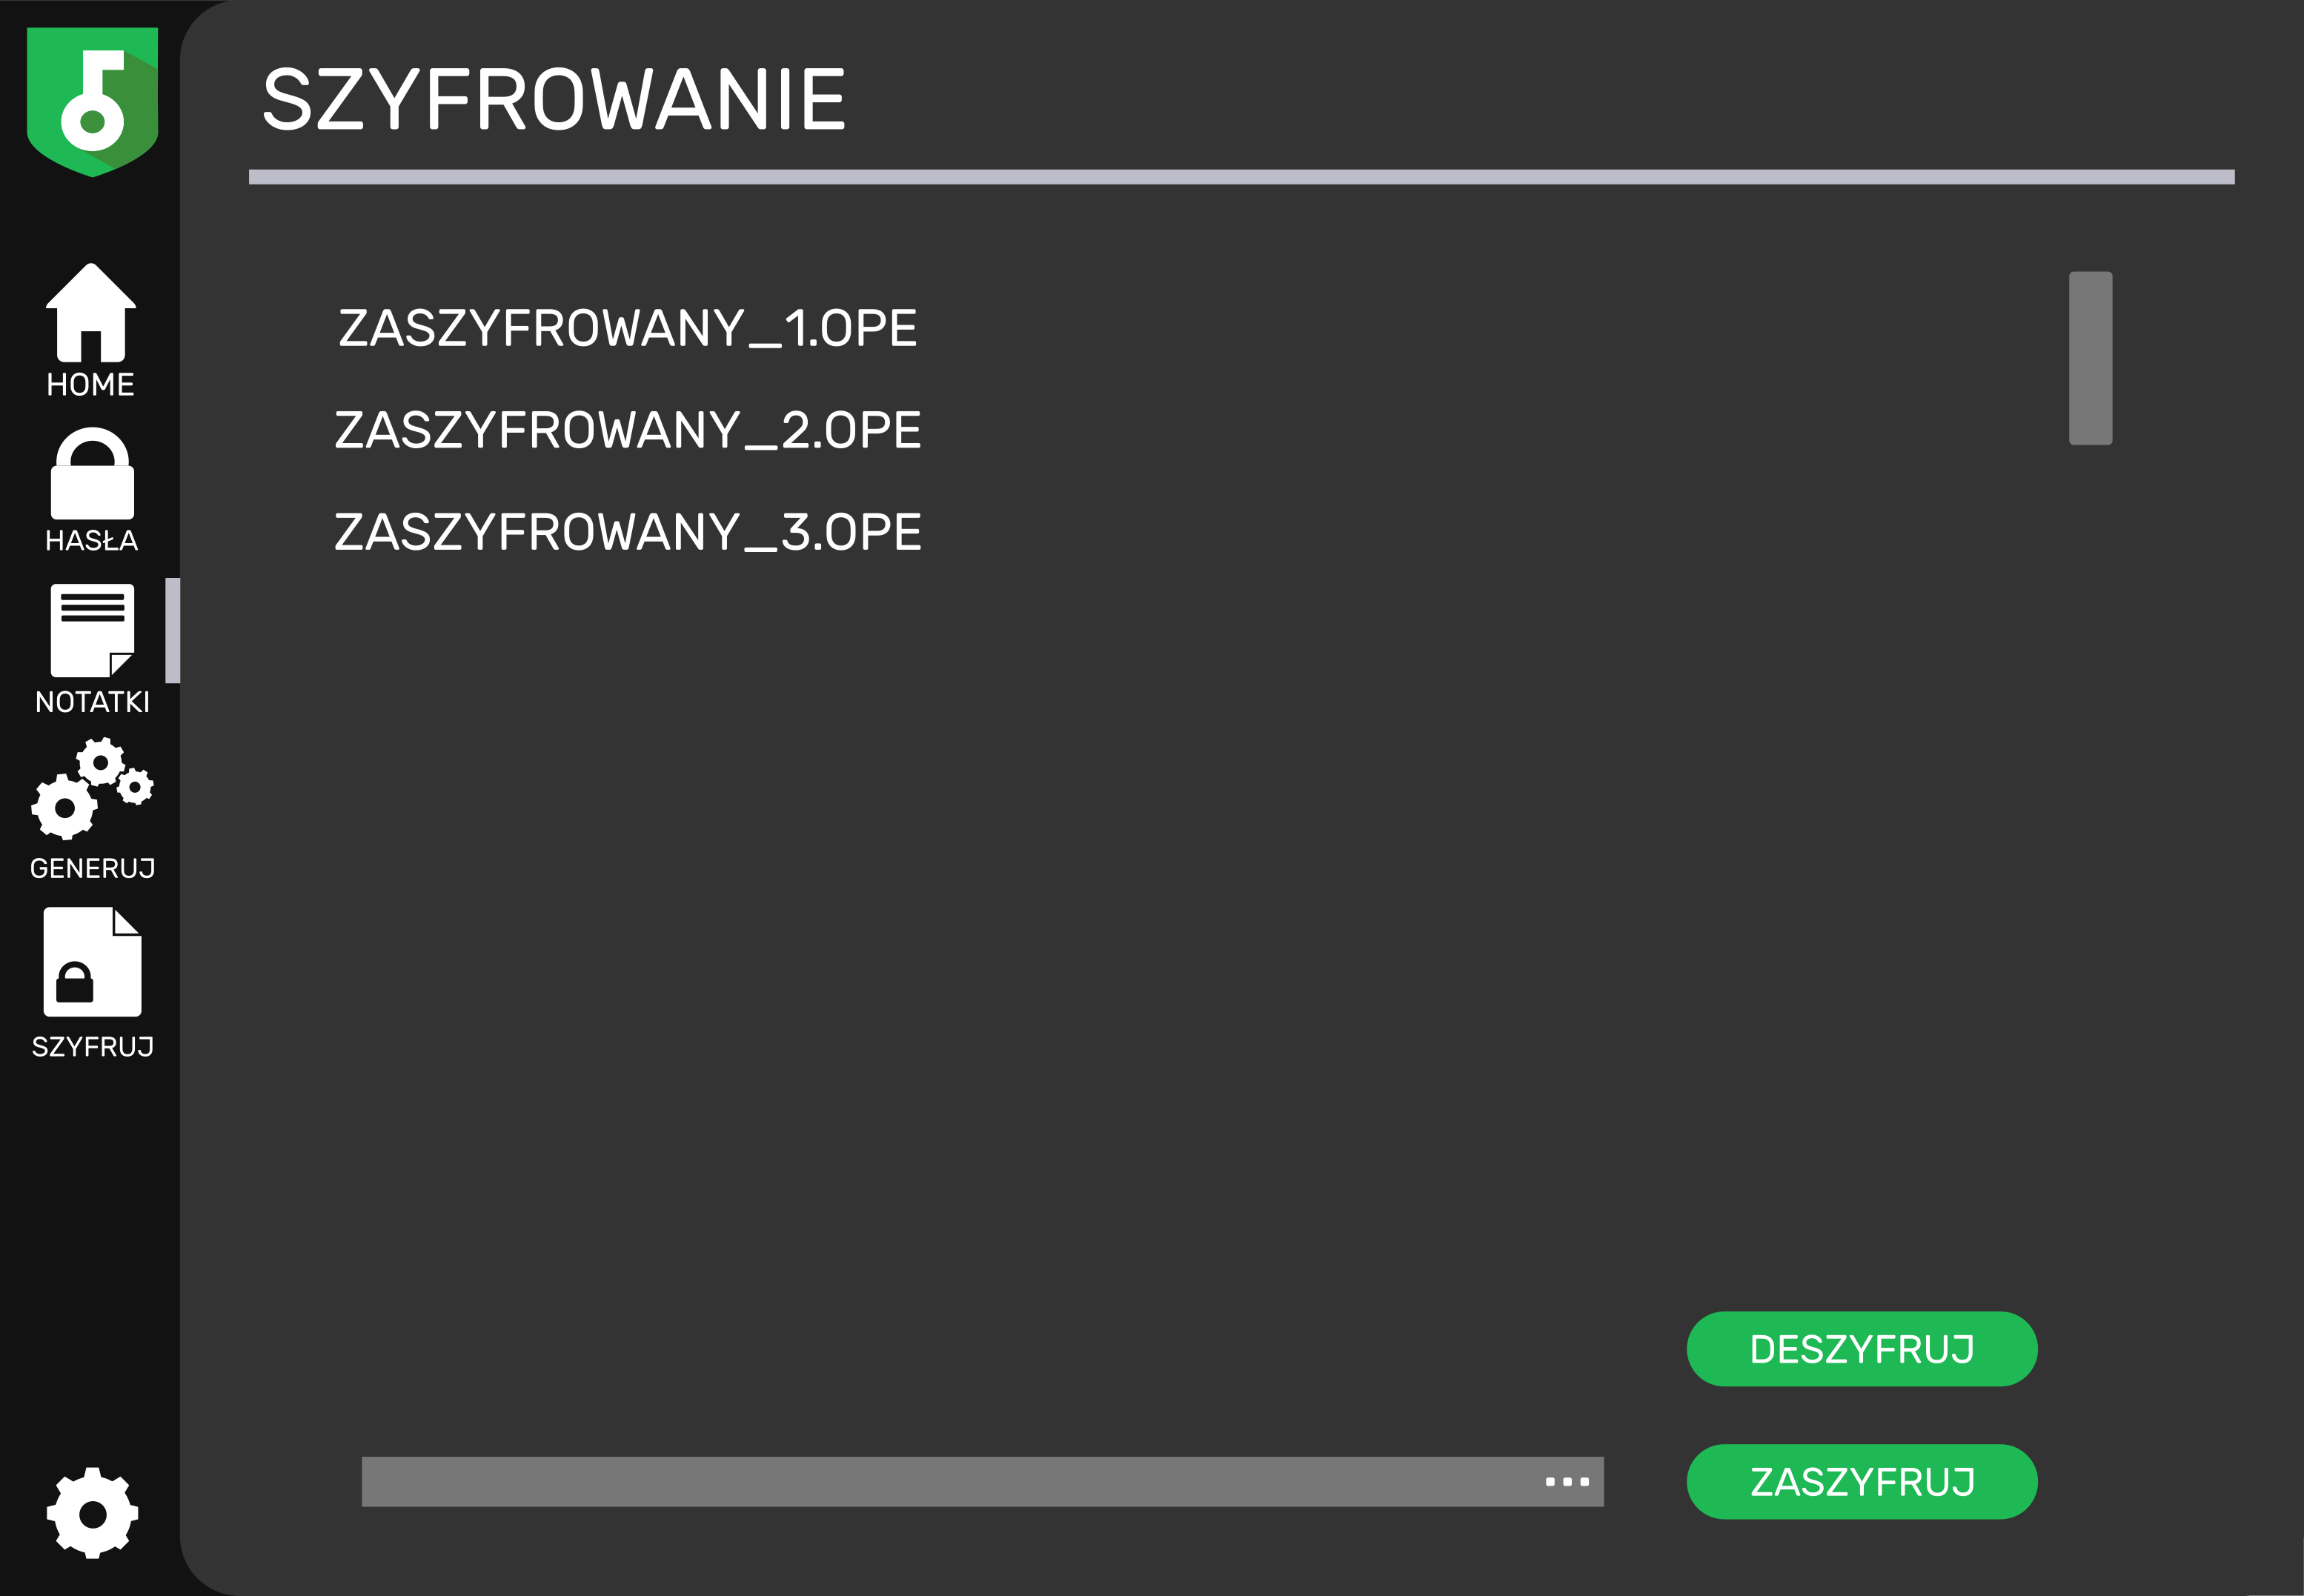
\includegraphics[width=1\textwidth]{img/ekran_szyfrowania.png}
    \caption{Ekran szyfrowania plików podanych przez użytkownika}
    \label{fig:szyfrowanie}
\end{figure}

\paragraph{}\textit{Pojedyncze elementy grafiki wektorowej i fonty użyte do przygotowania poglądowych rysunków pochodzą z otwartych źródeł. Licencje pozwalają na ich bezpłatne wykorzystanie (bez obowiązku podania autora) zarówno w projektach prywatnych jak i komercyjnych. Wszystkie powstałe do projektu wizualizacje są naszą autorską inwencją twórczą.}

\section{Testowanie}
\subsection{Ogólny przebieg testowania}
Do przetestowania kodu użyje narzędzi z biblioteki \textit{unittest}. Natomiast GUI przetestuje ręcznie podczas tworzenia aplikacji.
\label{end}

\end{document}